\documentclass[bibliography=totoc,listof=totoc,BCOR=5mm,DIV=12,oneside]{scrbook}
\usepackage[utf8]{inputenc}
\usepackage[T1]{fontenc}
\usepackage{lmodern}
\usepackage[ngerman]{babel}
\usepackage[T1]{fontenc}
\usepackage{microtype}
\usepackage{pifont}
\usepackage{amsmath}
\usepackage{hyperref}
\usepackage{booktabs}
\usepackage{subfigure} 
\usepackage{colortbl}
\usepackage{pdfpages}
\usepackage{graphicx}
\usepackage{enumitem}
\usepackage{threeparttable}
\usepackage{float}
\usepackage{multirow}
\usepackage{pdflscape}
%\usepackage{lscape}
\setlength{\parindent}{0em} 
\usepackage[citestyle=authoryear,natbib=true,style=alphabetic,backend=bibtex]{biblatex}
\usepackage{tabularx}

\newcommand*\adjust{\setlength\hsize{3\hsize+4\tabcolsep}} 

\addbibresource{lit.bib} 

\title{Eine gamifizierte Howto-App für Bachelorarbeiten}
\author{Tim-Pascal Lau}
\date{28.05.2018}
\begin{document}
\maketitle
\tableofcontents
\listoftables
\listoffigures

\chapter{Einleitung}
Für Studierende im letzten Semester eines Bachelorstudiengangs, umfasst die wesentliche Prüfungsleistung das Verfassen einer Bachelorarbeit.
Die Auseinandersetzung mit komplexen Problemstellungen stellt jedoch erfahrungsgemäß für viele Studierende eine große Herausforderung dar, welche sich aus dem erstmaligem Zusammenspiel von selbständigem und eigenverantwortlichen Arbeiten, sowie Problemlösen mittels erworbener Fach- und Methodenkenntnisse über einen längeren (in etwa dreimonatigen) Zeitraum ergibt.

\section{Motivation}
Im Verlauf des Studiums sollten Studierende folgendes Wissen und folgende Fähigkeiten erworben haben und zielgerichtet Anwenden können:
\begin{itemize}
\item Studiengang-spezifisches Grundlagenwissen
\item Wissensansammlung über fachspezifische Methoden und deren Eigenschaften
\item Fähigkeit, komplexe Probleme zu erkennen, zu strukturieren und systematisch mittels geeigneter Methoden zu bearbeiten
\end{itemize}
Wie bei Betrachtung der Umfrageergebnisse (siehe Anhang \ref{anhang:onlineUmfrageStudierendeErgebnisse}) anzunehmen ist, kommt es im Kontext von Bachelorarbeiten dennoch oftmals zu Schwierigkeiten, das erworbene Wissen und Fähigkeiten zielgerichtet auf reale Probleme anzuwenden und deren Ergebnisse zusammenhängend zu dokumentieren, da sich die Studierenden häufig nicht ausreichend vorbereitet fühlen.

\section{Lösungsansatz}
Ein möglicher im Rahmen dieser Bachelorarbeit zu verfolgender Lösungsansatz wäre es, eine Software zu entwickeln, welche unterstützend und wegweisend bei dem systematischen Vorgehen bei komplexen Problemstellungen fungieren könnte und diese den Studierenden zugänglich zu machen.
Hierbei soll es nicht darum gehen, den Studierenden die eigentliche Arbeit abzunehmen, sondern vielmehr darum, Studierende hinsichtlich Vorgehen und Methodenauswahl zielgerichtet zu unterstützen.

\section{Zielsetzung}
Mit einem solchen Ansatz soll es Studierenden ermöglicht werden, ihr gelerntes Wissen durch Fokussierung bestimmter Aufgaben und Zusammenhänge im Rahmen ihres eigenen Bachelorprojekts auf die Realität zu übertragen und somit einen motivierenden, sowie gleichermaßen fordernden Rahmen zu schaffen, um ihr Bachelorprojekt erfolgreich abzuschließen.

\section{Aufgabenbeschreibung}
Im Rahmen dieser Bachelorarbeit soll hierfür eine mobile Applikation entwickelt werden, die den Studierenden während der Dauer der Bachelorarbeit kontinuierlich "begleitet". Dabei sollen Gamificationansätze realisiert werden, welche motivierend im bei der Bearbeitung und dem Vorgehen der eigenen Bachelorarbeit wirken sollen. Dies soll beispielhaft für den Studiengang Informatik/Softwareentwicklung erfolgen. Eine Erweiterbarkeit für andere Studiengänge ist hierbei jedoch konzeptionell vorzusehen
Primäre Funktionen der Software ist Studierenden bei den folgenden Aufgaben begleitend zu unterstützen und fortwährend zu motivieren "am Ball zu bleiben":
\begin{itemize}
\item Brainstorming (zur Unterstützung der Ideenfindung für Bachelorarbeiten)
\item Recherche und Literaturverwaltung
\item Gliederung (unterschiedlicher Kategorien von Bachelorarbeiten, zum Beispiel mittels bewehrter Templates)
\item Zeitplanung/Fortschrittsverfolgung, sowie Erinnerungs- und Benachrichtigungsfunktion 
\item Problem-orientierte Anforderungsanalyse und deren Dokumentation
\item Problem-orientierte Methoden- und Tool-/Frameworkselektion und deren Dokumentation
\item Methoden-spezifische Aufbereitung von Ergebnissen
\item Problem-orientierte Nachweisführung und deren Dokumentation
\end{itemize}
Die Applikation soll mittels Flutter für Android und iOS entwickelt werden. Dabei soll erhoben werden, inwiefern sich Flutter für die Entwicklung solcher Apps eignet(Lessons Learned). 
Die im Rahmen der Aufgabenbeschreibung entstandenen Anforderungen werden durch die folgenden Teilaufgaben spezifiziert:
\begin{itemize}
\item Detaillierte Anforderungsanalyse oben angegebener Funktionen. Hierbei sind Studenten und Professoren des Studiengangs Informatik/Softwaretechnik geeignet einzubeziehen und relevante Literatur (insbesondere zu Gamification und Methoden der Informatik und des Softwareengineering) zu berücksichtigen.
\item Architekturentwurf der Anwendung (Erweiterbarkeit für andere Studiengänge ist konzeptionell vorzusehen)
\item Implementierung der Anwendung
\item Die Funktonsfähigkeit der App soll mittels Softwaretests geeignet nachgewiesen werden.
\item Die Nutzbarkeit der App soll systematisch evaluiert werden. Hierbei sind Studenten und Professoren des Studiengangs Informatik/Softwaretechnik geeignet einzubeziehen.
\item Dokumentation der oben angegebenen Schritte inklusive Bewertung der Nutzbarkeit des Frameworks Flutter für solche Arten von Apps.
\end{itemize}

\section{Ausblick auf die Bachelorarbeit}
\par In der folgenden Dokumentation der Bachelorarbeit werden verschiedene aufeinander aufbauende Prozesse, Teilschritte und Ergebnisse der Softwareentwicklung dokumentiert sein. Hierbei liegt die Priorität vor allem bei dem Pflegen der Nachvollziehbarkeit der dargestellten Informationen durch aufeinander aufbauende Kapitel und dem reflektieren der eigenen Gedankengänge.

\subsection{Beschreibung der Kernkomponenten}
\par Der Nachvollziehbarkeit halber empfiehlt es sich, Grundkenntnisse über die Basiskomponenten, wie dem Flutter Framework zu besitzen. Sollte dies nicht der Fall sein, so lassen sich in Kapitel \ref{chap:grundlagenkapitel} die nötigen Informationen nachlesen.

\subsection{Untersuchung des Problembereiches}
\par Das Kapitel \ref{chap:problemanalyse} stellt in detaillierter Ausführung und Beschreibung die Prozesse der Anforderungsermittlung und deren Auswertung, sowie Definition dar und legt somit wichtige Grundlagen und Anforderungen an die Software fest. Weiterhin werden im Laufe des Kapitels Einblicke in Strategien und Gedankengänge ermöglicht, welche zusätzliche Anhaltspunkte für die Nachvollziehbarkeit der weiteren Kapitel beitragen können.

\subsection{Konzeptvortellung der Applikation}
\par \ref{chap:konzept}


\subsection{Architektur der Software}
\par Alle Informationen zur Softwarearchitektur, zu den Entwurfsentscheidungen, sowie der Berücksichtigung der Erweiterbarkeit der Software, werden im Kapitel \ref{chap:architektur}  behandelt.

\subsection{Implementierung}
Informationen zur detaillierten Implementierung der in der Aufgabenbeschreibung definierten Funktionen, sowie die Umsetzung der Benutzeroberfläche, werden im Kapitel \ref{chap:implementierung} behandelt. Unter Einbezug beispielhafter Codeauszüge werden hier die Funktionsweisen der Software aufgeführt und beschrieben.

\subsection{Validierung und Verifikation}
Die Nachweisführung der Softwareanforderungen, der Usability-Anforderungen, sowie die Auswertung der Nützlichkeit der Verwendung des Frameworks Flutter bei der Entwicklung dieser App lassen sich im Kapitel \ref{chap:nachweisführung} nachlesen.

\subsection{Präsentation der Ergebnisse}
Abschließend folgt im Kapitel \ref{chap:ergebnisse} eine Zusammenfassung der erreichten Ergebnisse und eine Reflexion der Teilschritte, sowie die Abschlussbetrachtung des gesamten Projekts.


\chapter{Beschreibung der Kernkomponenten} \label{chap:grundlagenkapitel}

\section{Vorstellung des Frameworks Flutter}
Flutter ist ein von Google entwickeltes opensource Framework, welches auf die Entwicklung mobiler 2D-Applikationen für Android- und iOS-Betriebssysteme ausgelegt ist. Beworben wird Flutter durch das Hervorheben der Einfachheit der Benutzung, die schnell zu erreichenden Fortschritte bei der Implementierung von Softwarefunktionen, sowie den Gestaltungsmöglichkeiten der Benutzeroberfläche und den hochqualitativen Ergebnissen.

\subsection{Flutter Systemarchitektur} 
Das Flutter Framework besteht aus drei verschiedenen Basiskomponenten, welche im folgenden Abschnitt kurz erläutert werden.
\begin{itemize}
\item{\textbf{Flutter Engine}}

Die C/C++ basierte Flutter Engine, setzt sich aus verschiedenen Kerntechnologien zusammen. Zum einen die open source 2D Graphics Libary Skia\citep{Skia1}, welche seit 2005 zu Google gehört und zum anderen die Dart Virtual Machine.
\item{\textbf{Foundation Libary}}

Die Foundation Libary, welche in Dart geschrieben wurde, stellt Basisklassen und -funktionen zur Verfügung und dient der Konstruktion von Applikationen mittels Flutter
\item{\textbf{Design-specific Widgets}}

Das Flutter Framework stellt zwei verschiedene Arten von Widgets zur Verfügung, welche zugehörig zu den jeweiligen Design Sprachen von Google Material Design\citep{Mat1}, welche 2014 entwickelt wurde und die iOS Design kopierende Design Sprache Cupertino\citep{Cup1}.
\end{itemize}

		...
\section{Redux-Architektur}
\section{Gamification} \label{sec:grundlagenkapitelGamification}
Vergleiche \citep{Strahringer2017}57

\subsection{Bekannte Spiel-Design-Elemente} \label{sub:grundlagenSpielDesignElemente}
\par Im folgenden Kapitel werden die wichtigsten interaktiven Spiel-Design-Elemente \citep[vgl.]{blohm2013gamification} Vorgestellt und beschrieben. 
Vergleiche \citep[Kapitel 2.2.2 Analyse einzelner Spiel-Design-Elemente]{Sailer2016}

\par \bigskip \textbf{Dokumentation von Verhaltensweisen}
\par Durch die ständige Dokumentation der eigenen Verhaltensweisen, werden persönliche Fortschritte für den Anwender sichtbar gemacht. Diese Fortschritte können ein Gefühl von hoher Leistungsfähigkeit auslösen, da auf diese Weise ein Vergleich zu den bisherig erreichten Leistungen ermöglicht wird und somit bei Verbesserung der eigenen Leistung, der persönliche Fortschritt verdeutlicht werden kann.
\par \bigskip \textbf{Punkte}
\par Punktesysteme sind in ihrer Einfachheit eine weitverbreitete Form der Spiel-Design-Elemente, welche hauptsächlich eine Feedbackfunktion erfüllen. Diese Feedbackfunktion kann dem Spieler durch diverse weitere Möglichkeiten, wie zum Beispiel das Aufsteigen eine Levels, unterschiedlich stark verdeutlicht werden, weshalb Punkte häufig als Grundbestandteil von Gamification-Anwendungen auftreten. Weiterhin symbolisieren Punkte dem Spieler seinen derzeitigen Spielstand und bieten bei der Kombination mit Bestenlisten eine Vergleichsmöglichkeit zu anderen Spielern. In dieser Kombination können Punktesysteme also je nach Zielstellung auch Gewinner einer Herausforderung identifizieren.
\par In den zwei, in \citep{Sailer2016} behandelten, empirischen Untersuchungen \citep{mekler2013disassembling} und \citep{mekler2013points}, wurde nachgewiesen, dass der Einsatz von Punktesystemen, durchaus einen leistungsfördernden Effekt auf Spieler haben können.
\par \bigskip \textbf{Ranglisten}
\par \bigskip \textbf{Ränge, Levels, Reputationspunkte}
\par \bigskip \textbf{Gruppenaufgaben}
\par \bigskip \textbf{Zeitdruck, Aufgaben, Missionen}
\par \bigskip \textbf{Avatare, virtuelle Welten, virtueller Handel}


\begin{tabularx}{\textwidth}{l|l|X}
	\toprule
	\textbf{Spiel-Mechanik} & \textbf{Spiel-Dynamik} & \textbf{Motiv}\\ \midrule
	Dokumentation von Verhaltensweisen & Exploration & Wissbegierde\\
	Punktesysteme, Badges, Trophäen & Sammeln  & Leistung\\
	Ranglisten & Wettbewerb & Soziale Anerkennung\\ 
	Ränge, Levels, Reputationspunkte & Statuserwerb  & \\
	Gruppenaufgaben & Zusammenarbeit  & Sozialer Austausch\\
	Zeitdruck, Aufgaben, Missionen & Herausforderung & Kognitive Stimulation\\ 
	Avatare, virtuelle Welten, virtueller Handel & Entwickeln/Organisieren & Selbstbestimmung \\ 
	\bottomrule
\end{tabularx}
\captionof{table}{Übersicht der Spiel-Design-Elemente \citep[vgl.]{blohm2013gamification}}
\label{tab:spielDesignElemente}
\subsection{Nutzergruppen nach Bartle} \label{sub:nutzergruppenBartle}
\par Nach Bartle \citep{bartle1996hearts} werden vier verschiedene Nutzertypen voneinander unterschieden, welche im folgenden kurz erläutert werden.
\par Zudem werden den jeweils genannten Benutzergruppen die bekannten Spiel-Design Elemente ihrer Wirksamkeit bei der Steigerung der Motivation zugeordnet. (TODO)

\begin{itemize}
\item \textbf{Der Killer}
\par Die Killer legen den Fokus auf den Wettkampf und somit beruht ihre Motivationsquelle auf stark kompetitiv ausgeprägte Ursprünge. Sie fühlen sich dadurch motiviert, den Kontakt mit anderen Individuen im Rahmen eines Wettkampf zu überstehen und sich durch den eigenen Sieg gegenüber anderen Personen zu behaupten.

\item \textbf{Der Socialiser}
\par Die Gruppe der Socialiser sind immer auf der Suche nach sozialer Interaktivität. Ohne diese, können sie der Welt wenig bis keine Motivation abgewinnen. Die Spielwelt in der sie sich bewegen, ist vor allem nur der Mittel zum Zweck der Kommunikation. Der größte Stolz der Socialiser ist die Freundschaft und der Kontakt zu anderen Personen:

\item \textbf{Der Achiever}
\par Der Achiever ist im allgemeinen der Spielertyp, welcher sich auf das Erreichen von Leistungen konzentriert. Dieser wird so eingeschätzt, dass er die möglichst optimale geforderte Leistung erbringen will und er somit seine Motivation unter anderem auf das schrittweise Sammeln von Erfolgen und erfüllen von Aufgaben aufbaut.

\item \textbf{Der Explorer}
\par Die Explorer legen den Hauptfokus auf die Welt in der sie sich bewegen und möchten im Zusammenspiel mit dieser Spielwelt, durch immer wieder neu gestellte Aufgaben und erlebte Überraschungen alles entdecken, was es zu entdecken gibt. Sie sind sehr ambitioniert und empfinden Stolz für Ihr Wissen und Ihre Erfahrung in der Spielwelt. 
\par Die Explorer haben vor allem Interesse an der Spielwelt, und weniger an den Personen, die sie im Laufe der Erkundung treffen.
\end{itemize}

\begin{figure}[H]
	\centering
	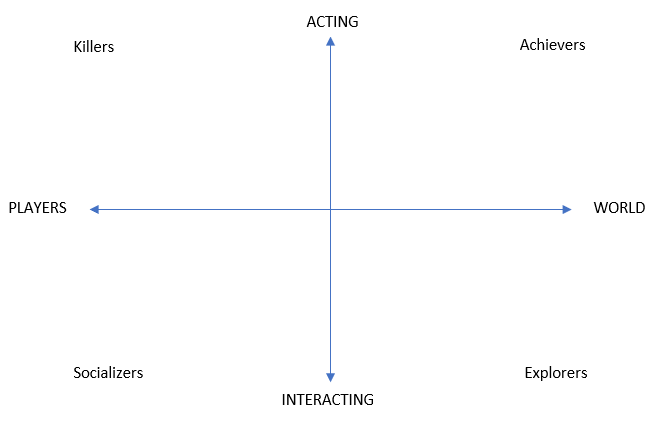
\includegraphics[width=0.85\textwidth, keepaspectratio]{Bilder/Diagramme/InterestGraphBartle.png}
	\caption{Interest Graph nach Bartle \cite{bartle1996hearts}}
	\label{img:interetGraphBartle}
\end{figure}

\chapter{Untersuchung des Problembereiches} \label{chap:problemanalyse}
\par In dem folgenden Kapitel werden die Rahmenbedingungen und die Analysestrategie zu den durchgeführten Befragungen von Professoren und Studierenden, aus dem Studiengang Informatik/Softwaretechnik der Fachhochschule Lübeck, dargestellt und die daraus resultierenden Ergebnisse und Erkenntnisse beider Seiten in zusammengefasster Form beschrieben. 
\par Weiterhin stellt die Diskussion dieser Ergebnisse und die aus den durchgeführten Befragungen abgeleiteten Anforderungen, an die zu entwickelnde Software, das Produkt der Anforderungsanalyse und somit den Ausgangspunkt für die gesamte Arbeit dar.

\section{Hypothese}
\par Die Auseinandersetzung mit komplexen Problemstellungen, wie die als abschließende Prüfungsleistung des Studiums zu erarbeitende Bachelorarbeit, stellt erfahrungsgemäß für viele Studierende eine große Herausforderung dar. Diese Herausforderung ergibt sich aus dem erstmaligen Zusammenspiel von selbstständigem und eigenverantwortlichem Arbeiten, sowie dem Problemlösen mittels erworbener Fach- und Methodenkenntnisse über einen längeren (in etwa dreimonatigen) Zeitraum.
Trotz des Verlaufs des Studiums, des angeeigneten Wissens und der somit zahlreich erworbenen Fähigkeiten, kommt es im Kontext von Bachelorarbeiten dennoch oftmals zu Schwierigkeiten, diesen Zusammenhang auf reale Probleme abzubilden und zu dokumentieren.

\newpage
\section{Identifikation der Interessengruppen}
\par Die folgende Tabelle \ref{tab:uebersichtInteressengruppen} bietet eine Übersicht, der im Rahmen des Projektes identifizierten Interessengruppen und welche Stellung diese zu dem Projekt, bezüglich Einfluss, Einstellung und Erwartungen einnehmen.

\medskip
\begin{center}
\scalebox{0.70}{
\begin{tabularx}{15cm}{l|l|l|X|X}
\toprule
\textbf{Bezeichnung} 
& \textbf{Einfluss} 
& \textbf{Einstellung} 
& \textbf{Erwartungen} 
& \textbf{Bemerkungen} 
\\ \midrule
	
\textbf{Studierende}
&  Hoch
&  Positiv
&  Erhoffen sich optimale Ergebnisse und weniger Fallstricke bei dem Bearbeiten der Bachelorarbeit und diesbezüglich eine insgesamt umfangreich ausfallende Hilfestellung.
&  Zielgruppe der zu entwickelnden Applikation
\\ \midrule

\textbf{AStA}
&  Hoch
&  Positiv
&  Erhoffen sich eine angemessene Förderung und Entlastung der Studierenden bei der Bearbeitung der Bachelorarbeit.
&  Sprachrohr und Interessenvertreter der Studierenden
\\ \midrule

\textbf{Betreuer}
&  Hoch
&  Positiv
&  Erhofft sich eine steigende Bereitschaft der Studierenden im Rahmen des Bachelorseminars Beiträge zu erbringen, sowie eine steigende Qualität der Vorbereitung, Bearbeitung und Fertigstellung von Bachelorarbeiten.
&  Leitet das Bachelorseminar, hat somit direkten Kontakt mit der Zielgruppe und trägt wichtige Erfahrungswerte bezüglich der Probleme der Studierenden mit sich.
\\ \midrule

\textbf{Professoren}
&   Hoch
&   Positiv
&   Erhoffen sich eine steigende Qualität der Bearbeitung der Bachelorarbeit, sowie eine Entlastung bei dem Betreuen von Studierenden, hinsichtlich sich wiederholenden Erklärungen und weiteren Trivialitäten.
&  Tragen wichtige Erfahrungswerte durch den detaillierten Einblick als Betreuer von Bacheloranden, sowie dem Bewerten von Bachelorarbeiten mit sich.
\\ \midrule

\textbf{Präsidium}
&  Mittel
&  Positiv
&  Erwarten eine Steigerung der Leistung der Studierenden an der FH-Lübeck
&  Machtpromotor der FH-Lübeck
\\ \midrule
\bottomrule
\end{tabularx}}
\begin{tablenotes}
\item  
\end{tablenotes} 
\captionof{table}{Übersicht der Interessengruppen}
\label{tab:uebersichtInteressengruppen}
\end{center}

\newpage
\section{Wahl der Analysestrategie}
\par Um den Problembereich zu ermitteln und somit eine Analysegrundlage zu erschaffen, werden Personengruppen der Fachhochschule Lübeck, durch verschiedene Befragungs- und Analysemethoden in das Projekt miteinbezogen. Dies soll einen detaillierten Einblick in die Sichtweisen der unterschiedlich beteiligten Personen und Interessengruppen ermöglichen und somit eine Grundlage für das Verständnis der aktuellen Situation bilden.

\par Als primäre Einflussgeber, welche in die Entwicklung der Applikation stark eingebunden werden, wurde die Gruppe der Professoren, sowie die Gruppe der Studierenden identifiziert. Diese Entscheidung wurde aufgrund der im Rahmen der Bachelorarbeit existierenden unterschiedlichen Sichtweisen, sowie der unmittelbaren Berührung des Problembereiches der Beteiligten und den unterschiedlichen Erfahrungsständen von Betreuern und Bacheloranden getätigt (siehe Abbildung \ref{tab:uebersichtInteressengruppen}). Darüber hinaus handelt es sich bei den Studierenden um die Zielgruppe und potentiellen späteren Anwender, weshalb die Aufnahme der Probleme und Meinungen der Studierenden als essenziell angesehen wird. 

\par \bigskip \textit{Anmerkung: Der Inhalt von Abbildung \ref{img:analysestrategie} ist in detaillierter Form, als Sequenzdiagramm in UML-Notation, im Anhang zu finden (siehe \ref{anhang:datenerhebungStrategieAktivitätsdiagramm}). Aus Gründen der Übersicht wurde hier jedoch darauf verzichtet}

\bigskip
\begin{figure}[H]
	\centering
	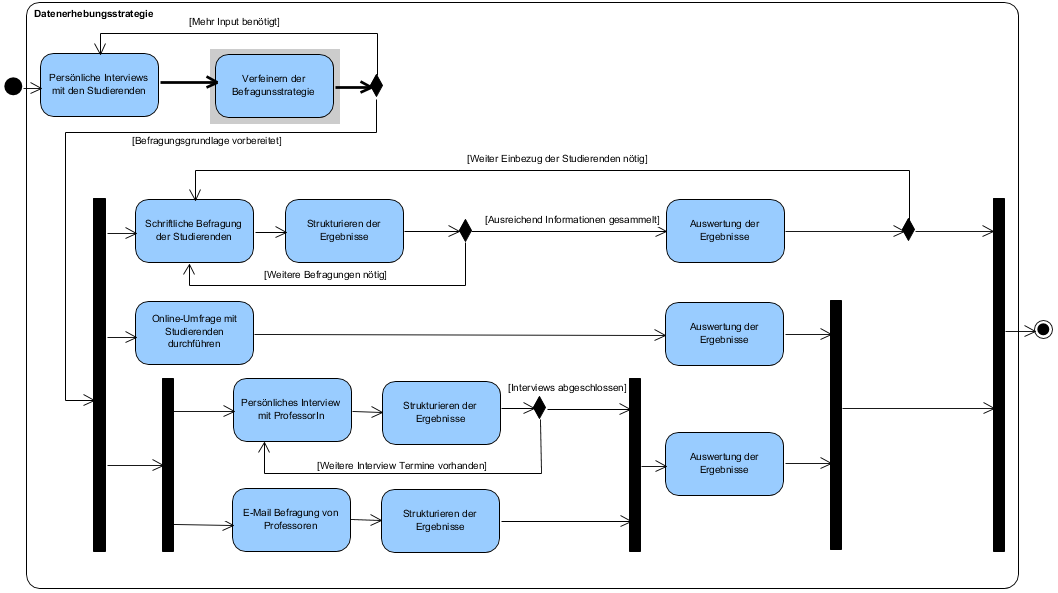
\includegraphics[width=1\textwidth, keepaspectratio]{Bilder/Diagramme/Analysestrategie.png}
	\caption{Beschreibung der Analysestrategie}
	\label{img:analysestrategie}
\end{figure}

\par Durch die initial ausgeführten Gespräche mit den Studierenden ließen sich Erkenntnisse über den Umfang des Problems gewinnen. Auf Grundlage dieser Erkenntnisse wurde die weitere Analysestrategie verfeinert und für die Umsetzung durch die Erstellung von Fragekatalogen und Interview-Leitfaden vorbereitet (siehe Abbildung \ref{img:analysestrategie}), welche im folgenden Verlauf beschrieben werden.
\par Die Interviews mit den Studierenden sollen somit als Grundlage zur Konzeption und Design weiterer Befragungsstrategien dienen und stellen in diesem Umfang einen Ausgangspunkt für die Problemanalyse dar. Weiterhin wurden die gewählten Interviewpartner bei Zustimmung, über das gesamte Projekt und nach Absprache, auch in die Evaluation der Applikation miteinbezogen.
\par\medskip Durch das Durchführen von Gruppeninterviews, sollen die Studierenden zu Diskussionen angeregt sein, welche von dem Leiter des Interviews durchaus auch motiviert werden können. Dies hat den Zweck, die Situation und die Rolle der Studierenden für den Interviewer erkenntlich zu machen.  Diese persönlichen Interviews dienen in erster Linie also nicht der Erhebung konkreter Daten, sondern als erster Berührungspunkt mit dem Problembereich und in diesem Rahmen als strategischer Orientierungspunkt für mich, als Projektleiter.

\subsection{Einbezug der Professoren}
\par Für die Interessengruppe der Professoren aus dem Fachbereich Informatik, ist als Grundlage der Datenerhebung einerseits das Durchführen von Einzelinterviews mit einer ausgewählten Gruppe von Professoren vorgesehen, während eine weitere Gruppe von Professoren schriftlich per E-Mail befragt wird (siehe Abbildung \ref{img:analysestrategie}). Dies bietet sowohl den Zugriff auf die unmittelbaren Erfahrungen der einzelnen Professoren als Spezialisten in den jeweiligen Fachgebieten, als auch auf die Erfahrungen der Professoren in der Position eines Betreuers und Ansprechpartners für Bacheloranden. 
\par Durch das Durchführen von Einzelinterviews wird ermöglicht, die Erwartungen seitens der Professoren an die Bacheloranden im Detail zu identifizieren und die, in dieser Hinsicht priorisierten inhaltlichen und methodischen Aspekte bei der Bearbeitung einer Bachelorarbeit herauszuarbeiten. Die Aufteilung auf Einzelinterviews und E-Mail Befragungen bietet den Vorteil, beide Strategien simultan zu verfolgen und nach Abschluss der Datenerhebung sowohl die detaillierten Einzelinterviews, als auch die oberflächlicher ausfallenden E-Mail Antworten in bereits dokumentierter Form vorliegen zu haben, um diese dann auszuwerten.

\subsection{Einbezug der Studierenden}
\par Nach Absprache mit den intervieweten Studierenden, werden diese weiterhin per schriftlicher Befragung in die Entwicklung des Projektes, unter ergänzender Zunahme anderer Studierender, eingebunden.
\par In diesem Umfang werden die teilnehmenden Studierenden mittels Bildern, Fragen und Gestaltungsmöglichkeiten der Applikation regelmäßig über den aktuellen Stand der Entwicklung informiert. Auf diese Weise sollte es möglich sein, ein breites, jedoch persönliches Feedback zu erhalten, da sich die Einbindung der Studierenden auf diese Weise sehr gut automatisieren lässt. Wesentlich dabei ist auch die Hoffnung, dass die Reaktionsfreudigkeit der Studierenden höher ausfällt, als für die im Vergleich existierende Alternative der zeitaufwändigeren persönlichen Interviews.
\par Durch die Durchführung der schriftlichen Befragung wird der Ablauf bereits dokumentiert und der Fragesteller, sowie die Studierenden haben jederzeit die Möglichkeit Fragen und Anregungen zu teilen.
\par Miteinbezogen werden vorzugsweise alle Studierende der oberen Semester, unabhängig davon, ob sie sich vor Beginn, während der Bearbeitung oder nach Abschluss der Bachelorarbeit befinden, da die unterschiedlichen Sichtweisen und Erfahrungsstände wichtige Impulse für die Entwicklung der Applikation geben könnten.
\par\medskip Des weiteren wird eine Online-Umfrage den Teil der Datenerhebung darstellen, der quantitative Ergebnisse erzielen soll und deren Aussage somit eine nicht durch die schriftlichen Befragungen abgebildete Menge darstellt.
\par Die Umfrage richtet sich nicht nur an die Studierenden des Studiengangs Informatik/Softwaretechnik, sondern im Sinne der Erweiterbarkeit für andere Studiengänge, an Studierende im Allgemeinen, welche sich ab dem 4. Semester bereits in der zweiten Hälfte des Studiums befinden und somit schon einen ein­schätz­baren Erfahrungsschatz aufgebaut haben.

\section{Ergebnisse der Professoren}
\par Im Folgenden sind die gewonnenen Eindrücke und Kenntnisse der Einzelinterviews mit den Professoren des Fachbereichs Informatik durch Themenkategorien geordnet und in zusammengefasster Form dokumentiert.
\par Es haben insgesamt sechs Professoren an persönlichen Einzelinterviews teilgenommen, wobei es für fünf Interviews gestattet wurde, eine Tonaufzeichnung anzufertigen.
\par\medskip Des Weiteren wird auch eine schriftliche Befragungen miteinbezogen, die jedoch das gleiche Fragespektrum wie die Interviews einnimmt.
\par\bigskip \textbf{Allgemeine Informationen}
\par Der zeitliche Rahmen der fünf aufgezeichneten Interviews erstreckt sich über einen Zeitrum von etwa 30 bis 45 Minuten. Für die Auswertung der aufgezeichneten Interviews wurden die Aussagen der Interviewpartner, auf Grundlage der vorliegenden Audioaufnahmen, unter Berücksichtigung des Kontextes aufbereitet und werden nachfolgend dargestellt. Ein weiteres Einzelinterview, welches nicht aufgezeichnet wurde, erstreckte sich über einen Zeitraum von 75 Minuten. Für dieses Interview wurden lediglich begleitende Feldnotizen angefertigt. Diese Feldnotizen wurden im Anschluss des Interviews aufbereitet und fließen zusammen mit den Ergebnissen der schriftlichen Befragung in die folgende Beschreibung ein.
\par\medskip Die gewählten Kategorien ergeben sich aus dem gewählten Auswertungsverfahren, was sich an der qualitativen Inhaltsanalyse nach Mayring\citep{Mayring2015} orientiert und basieren in diesem Kontext auf die gemäß des Verfahrens herausgearbeiteten Codings.

\par \bigskip Die komplette Zusammenfassung ist im Anhang dieses Dokuments zu finden (siehe Anhang \ref{anhang:interviewProfessorenAuswertung})). Weiterhin sind auch die Interviews mit den einzelnen Professoren in transkribierter Form im Anhang zu finden (siehe Anhang \ref{anhang:interviewProfessorenTranskripte}).

\newpage
\subsection{Art der Arbeit}
\par Im Laufe der Interviews wurden verschiedene Typen von Arbeiten versucht zu identifizieren. Dabei geht es vor allem darum, die Vielfalt der typischen Arbeiten des Studiengangs Informatik/Softwareentwicklung zu erfassen und somit einen Überblick über die Situation zu bekommen.
\par \medskip Als im allgemeinen auftretenden Arten der Arbeit wurden die Klassen \textit{Entwickelnde Arbeit}  und \textit{Evaluierende Arbeit} identifiziert. Weiterhin gibt es auch \textit{Reine Literaturarbeiten}, welche in dem Studiengang Informatik/Softwareentwicklung jedoch nicht oder nur in einem sehr geringen Vorkommen auftreten.

\par\medskip Es folgt eine stichpunktartige Ausführung der gewonnenen Erkenntnisse:


\par \bigskip \textbf{Konstruktiv/Entwickelnd - Durchlauf des Softwareentwicklungszyklus}
\par \medskip Die Art der konstruktiven/entwickelnden Arbeiten, befassen sich hauptsächlich mit dem Durchlaufen des Softwareentwicklungszyklus. Im Rahmen der Bachelorarbeit werden die verschiedenen Aufgaben der Softwareentwicklung, je nach Schwerpunkt der Arbeit, mehr oder weniger intensiv von dem Bacheloranden bearbeitet und beschrieben.
\par \medskip Typischer fachlicher Inhalt einer solchen Arbeit könnten sein:
\begin{itemize}
\item[\textbf{1.}] Anforderungsanalyse
\item[\textbf{2.}] Entwurf einer Softwarearchitektur
\item[\textbf{3.}] Implementierung eines Softwareprototyps
\item[\textbf{4.}] Evaluation des Softwareprototyps
\end{itemize}

\par \medskip Typische Aufgabenstellungen:
\begin{itemize}
\item Entwicklung einer mobilen Applikation zur Interpretation von Bildmaterial.
\item Entwicklung einer mobilen Applikation zur Steigerung der Bereitschaft bei Senioren und Seniorinnen, Fitnessaktivitäten auszuführen unter Einbezug von  Gamificationelementen.
\item Entwicklung einer Software zur Optimierung der täglichen Arbeitsabläufe in Unternehmen A.
\end{itemize}

\par \medskip Ein weiterer wichtiger Aspekt sind die möglichen Interessenunterschiede zwischen dem externen Unternehmen und dem internen Betreuer der Fachhochschule, welche einen Einfluss auf die Inhalte der Bachelorarbeit haben können. Externe Unternehmen sind tendenziell eher an dem resultierenden Ergebnis interessiert, während die internen Betreuer darüber hinausgehend einen hohen Wert auf nachvollziehbare Methodik, Herangehensweise, sowie Planung und dem sauberen wissenschaftlichen Arbeiten legen und somit ein  hohes Interesse an dem Gesamtprozess haben.

\newpage
\par \bigskip \textbf{Analytisch/Evaluierend - Vergleich, Auswertung und/oder Nachweis eines Aufgabengegenstandes}
\par \medskip Die Art der analytisch/evaluierenden Arbeiten, beinhalten hauptsächlich die Analyse und Auswertung eines Aufgabengegenstandes oder mehrerer verschiedener Aufgabengegenstände. Es wird der gesamte Weg der Analysestrategie, der Durchführung der Analyse und der Auswertung behandelt.
\par \medskip Typischer fachlicher Inhalt einer solchen Arbeit könnten sein:
\begin{itemize}
\item[\textbf{1.}] Erstellen eines Kriterienkatalogs
\item[\textbf{2.}] Aufbau des Experiments
\item[\textbf{3.}] Durchführung des Experiments
\item[\textbf{4.}] Evaluation und Ergebnisauswertung
\end{itemize}

\par \medskip Typische Aufgabenstellungen könnten sein:
\begin{itemize}
\item Evaluation der Gesichtserkennungsdienste von Unternehmen A, Unternehmen B und Unternehmen C.
\item Untersuchung des Verhaltens einer neuen Technologie A, im Vergleich mit einer alten Technologie B.
\item Datenbankanalyse unter Anwendung von Machine-Learning-Alrogithmen
\end{itemize}

\par \bigskip \textbf{Reine Literaturarbeiten}
\par Reine Recherchierende Arbeiten finden in dem Studiengang Informatik/Softwareentwicklung aufgrund dem geringen Interesse seitens der Studierenden kaum statt und werden aus Gründen der Vollständigkeit lediglich erwähnt und nicht ausgeführt.

\newpage
\subsection{Erwartungen an den Bacheloranden}
\par Im Laufe der Interviews wurden die Professoren hinsichtlich Ihrer Erwartungen an die Bacheloranden befragt und haben in diesem Rahmen häufig gleiche oder ähnliche Punkte ausgeführt. Aus diesem Grund werden im folgenden Verlauf die Meinungen der befragten Professoren aus der Sicht als Betreuer, unter den jeweiligen Aspekten als zusammengefasstes Meinungsbild wiedergegeben.

\par\medskip Es folgt die Ausführung der gewonnenen Erkenntnisse:

\par \bigskip \textbf{Selbständiges Arbeiten}
\par Das selbstständige Arbeiten und Vorgehen ist eines der am häufigsten genannten Erwartungen, welches sich in unterschiedlichen Punkten zum Ausdruck bringen lässt. Dazu zählt vor allem das selbständige kommunizieren von Ergebnissen und das Einholen von Feedback, sowie die Transparenz bei Problemen oder Schwierigkeiten, um sich Hilfe von dem Betreuer zu holen. Es wurde mehrfach betont, dass es im Allgemeinen nicht die Aufgabe des Betreuers ist, nachzufragen und aufzufordern. Das Einbinden des Studierenden in die Erarbeitung der Aufgabenstellung ist ein häufig genannter Punkt, welcher bereits frühzeitig Engagement des Studierenden erfordert.
\par Des Weiteren stellt das Selbstständige Einarbeiten in die Probleme, die Auswahl geeigneter Methoden und Werkzeuge ein wesentlicher Inhalt der Arbeit dar.
\par \bigskip \textbf{Die Vorgehensweise}
\par Sehr häufig wird betont, dass die Vorgehensweise hinsichtlich der wissenschaftlichen Arbeitsweise von essenzieller Bedeutung ist. In diesem Rahmen soll der Studierende auch zeigen, dass er in der Lage ist große Probleme systematisch in Teilprobleme zu zerlegen und diese unter Berücksichtigung der im Studium vermittelten Methoden, Modelle und Techniken zu bearbeiten. Sehr wichtig ist dabei das vorausschauende Planen von Teilprozessen, wie beispielsweise das Evaluieren der Ergebnisse. Dies sollte von Anfang an berücksichtigt werden und die in diesem Rahmen getroffenen Entscheidungen sollten nachvollziehbar erklärt werden können. Dazu zählt weiterhin das Erstellen eines Zeitplans, welcher sich über die Zeit jedoch durchaus verändern kann. Es wird sehr viel Wert darauf gelegt, zu sehen, dass die Studierenden einen weiten Blick auf das gesamte Projekt entwickeln und pflegen.
\par \bigskip \textbf{Der Literaturteil}
\par Es wird betont, dass vor allem Wert auf einschlägige Quellen Wert gelegt wird. In diesem Umfang ist es wichtig, dass die Studierenden Literaturquellen verwenden sollten, die bereits eine anerkannte längere Gültigkeit besitzen. Weiterhin sollten die Studierenden über den Umfang von Grundlagenliteratur hinaus blicken und je nach Themengebiet und Arbeitsstand spezifischere Fachliteratur in die Arbeit einbeziehen. Dies kann auch bedeuten, dass auf wissenschaftliche Papiere und Primärquellen verwiesen werden soll. Je nach Thema und Aufgabenstellung kann der Literaturteil mehr oder weniger Umfangreich ausfallen, welches sich mit dem praktischen Teil der Arbeit ausgleichen kann.

\newpage
\par \bigskip \textbf{Der praktische Teil}
\par Im Allgemeinen soll der praktische Teil den Umfang der Aufgabenstellung abdecken und gegebene und/oder erhobene Anforderungen erfüllen. Je nach Thema und Aufgabenstellung der Arbeit nimmt dieser Teil einen höheren oder niedriger ausfallenden Umfang ein.
Der Studierende soll bei der praktischen Bearbeitung der Aufgabe zeigen, das er in der Lage ist, das im Studium gelernte Wissen, die kennengelernten Methoden und deren Ausführung umzusetzen. 
\par \bigskip \textbf{Das Ergebnis der Bachelorarbeit}
\par Grundsätzlich soll die Bachelorarbeit aus zwei Teilen von Leistungen bestehen. Die von dem Studenten durchgeführte Literaturarbeit nimmt einen Teil der Arbeit ein, während die eigenständige praktische Leistung den anderen Teil erfüllt. Der Umfang der jeweiligen Anteile kann dabei je nach Themengebiet und Aufgabenstellung stark variieren.
\par Das Ergebnis der Bachelorarbeit, welches sich je nach Art der Arbeit voneinander stark unterscheiden kann, soll wissenschaftlich erarbeitet und somit nachvollziehbar und belegbar sein, sowie im Optimalfall die Aufgabenstellung erfüllen. Es kann jedoch auch vorkommen, dass das angestrebte Ziel aus verschiedenen Gründen nicht erreicht wurde. Dies muss nicht bedeuten, dass es zu einer schlechten Bewertung der Bachelorarbeit kommt, sofern der Grund oder die Erkenntnis über ein bestimmtes aufgetretenes Problems belegbar und nachvollziehbar dokumentiert ist.

\newpage
\subsection{Häufig auftretende Probleme}
\par Es stellte sich im Verlauf des Interviews heraus, dass unterschiedliche Studierende immer wieder mit gleichen oder ähnlichen Problemen zu kämpfen haben. Im folgenden Verlauf werden diese genannten Probleme in aufbereiteter Form stichpunktartig beschrieben.

\par \medskip Es folgt die Ausführung der gewonnenen Erkenntnisse:

\par \bigskip \textbf{Zeitmanagement}
\par Als am häufigster genannter Aspekt ist das mangelhafte Zeitmanagement der Studierenden. Im Laufe der Bearbeitung der Bachelorarbeit kommt es häufig zu der Unterschätzung des nötigen  Zeitaufwandes, besonders hinsichtlich des Schreibens der Dokumentation. 
\par Viele Studierende schieben das Schreiben der Dokumentation auf einen späteren Zeitpunkt und geraten im späteren Verlauf der Bearbeitungszeit somit unter Zeitdruck. Die Betreuer haben unter diesen Umständen wenig Möglichkeiten, rechtzeitiges und hilfreiches Feedback zu liefern. Es wird häufig empfohlen, frühzeitig mit dem Schreiben anzufangen und dies begleitend zum Arbeitsfortschritt die Dokumentation an mehreren Stellen wachsen zu lassen. Trotz vieler Hinweise seitens der Betreuer, kommt es in diesen Belangen häufig zu starken Problemen.
Das Problem des mangelnden Zeitmanagements äußert sich unter anderem auch darin, dass die Studierenden sich bei der Bearbeitung in Details verlieren, da sie die Schwerpunkte der Arbeit nicht erkennen.
\par \bigskip \textbf{Wissenschaftliches Arbeiten}
\par Die Studierenden erfassen teilweise nicht die Bedeutung des wissenschaftlichen Arbeiten. Es kommt immer wieder zu Schwierigkeiten und Unklarheiten über den eigentlichen Umfang der Arbeit und wodurch sich das wissenschaftliche Arbeiten auszeichnet. Oft wird der falsche Umgang mit Literatur und Quellen als negatives Beispiel genannt.
\par Ein Kritikpunkt ist, dass es gibt in dem Studiengang Informatik/Softwareentwicklung keinen Kurs gibt, welcher die Studienenden auf das wissenschaftliche Arbeiten vorbereitet. In einigen Wahlpflichtmodulen werden diesbezüglich zwar Ansätze im Rahmen von Projekten integriert, jedoch gilt dies somit nur für die an dem Wahlpflichtmodul teilnehmenden Studierenden und steht auch nicht im Fokus der Projektarbeit.
\par \bigskip \textbf{Kommunikation}
\par Kommunikation und Transparenz ist ein weiteres angesprochenes Problem. Es kommt vor, dass Studierende und Betreuer unterschiedliche Ansichten über die Zusammenarbeit haben, welche sich dadurch äußern, dass die Studierenden auf Forderungen bezüglich Leistungen oder Ergebnissen der Betreuer warten oder aus sich sogar aus diversen Gründen nicht trauen, ihren aktuellen Arbeitsstand oder ihre Probleme mit dem Betreuer zu teilen. 
\newpage
\par \bigskip \textbf{Die Vorbereitung der Studierenden}
\par Bei der Vorbereitung der Studierenden nennen die beteiligten Interviewpartner unterschiedliche Aspekte, welche zum einen das mangelhafte selbständige Informieren der Studierenden kritisiert, andererseits jedoch auch eine optimaler zu gestaltende Vorbereitung der Studierenden seitens der Fachhochschule für den Studiengang Informatik/Softwareentwicklung.
\par \medskip Das angebotenen Bachelorarbeit Seminar wird positiv erwähnt, da es einen positiven Einfluss auf die Arbeit der Studienenden hat. Es müssen weniger Aspekte einer Bachelorarbeit erklärt werden, jedoch müssen viele Aspekte mehrfach wiederholt werden. 
\par Es wird betont, dass auch viele Informationsmaterialien im Lernraum der Fachhochschule Lübeck zu finden sind, auf die auch oft hingewiesen wird, jedoch von den Studierenden nicht in dem Umfang beachtet werden, für den die Materialien gedacht sind. Dabei wird unter anderem auch kritisiert, das die Informationsmaterialien teilweise schwer auffindbar sind, da sie nicht an einer zentralen Stelle, sondern verteilt im Lernraum liegen. 
\par Weiterhin wird jedoch auch betont, dass die Studierenden zu wenig Engagement aufbringen, sich trotz vieler Möglichkeiten selbstständig zu informieren. 

\subsection{Die Applikation - Wünsche und Anregungen}
\par In den Interviews wurden die Professoren nach ihren persönlichen Wünschen, Ideen und Anmerkungen bezüglich der Applikation gefragt. Es folgt die Ausführung der aufgenommenen Wünsche und Ideen.

\par \bigskip \textbf{Neuer Kanal zu den Studierenden}
\par Es wird der Wunsch geäußert, dass die Applikation verwendet werden kann, um in zentraler Form konkrete interne oder externe Bachelorarbeit-Themen, sowie Beispielthemen angeben zu können, da dies an der Fachhochschule Lübeck bisher nicht ermöglicht ist.
\par \bigskip \textbf{Plattform als Informationsquelle}
\par Es besteht der Wunsch, die im Lernraum vorliegenden Informationsmaterialien, durchaus auch in aufbereiteter Form, durch die Applikation den Studienreden zugänglicher zu machen.
\par \bigskip \textbf{Applikation zur Unterstützung des Zeitmanagements}
\par Es wird der Wunsch geäußert, die Studierenden bei dem Zeitmanagement, unter anderem durch Erinnerungen, zu unterstützen. In diesem Rahmen wird der Vorschlag eingebracht, möglichst detaillierte Beschreibungen von Arbeitspaketen in dem Tool zu verlangen, damit die Studierenden dazu gezwungen sind, sich rechtzeitig mit der Aufwandseinschätzung zu beschäftigen.


\newpage
\subsection{Die Applikation - Chancen und Risiken}
\par In jedem Interview bekamen die Professoren abschließend die Möglichkeit, ihre Erwartungen an eine solche Applikationen auszuführen und besonders auf die, aus ihrer Sicht mögliche Chancen und Risiken einzugehen. 
\par \bigskip Diese Anmerkungen werden im folgenden Verlauf zusammengefasst dargestellt:
\par \bigskip \textbf{Chancen}
\begin{itemize}
\item Die Applikation als neuer Kanal für die Studierenden, der dafür dienen kann, dass Studierende sich besser informieren können. Dies wird besonders in Bezug auf die Formalien einer Bachelorarbeit betont, da viele Studierende gar nicht wissen was die Rahmenbedingungen einer Bachelorarbeit sind oder welche Regeln und Anforderungen es überhaupt gibt.
\item Die Applikation kann im Gegensatz zum Bachelorseminar begleitend zu der eigenen Bachelorarbeit genutzt werden kann. Dies kann dafür sorgen, dass die Aufnahmebereitschaft der Studierenden für Tipps, Empfehlungen und weiteren Aspekten gesteigert wird, da sie sich zu diesem Zeitpunkt mit dem Problem konfrontiert sehen und somit der Lerneffekt am höchsten ist. In diesem Ansatz wird auch die Chance erkannt, dass der Fokus der Studierenden zum richtigen Zeitpunkt auf bestimmte wichtige Fragen gelenkt werden können und somit grobe Fehler minimiert werden können.
\item Besseres Zeitmanagement der Studierenden und die somit geförderten organisatorischen Fähigkeiten der Studenten.
\item Die App könnte Probleme im Projektmanagement und bei der Gestaltung der Dokumentation minimieren.
\item Das Senken des Beratungsaufwandes für Professoren und somit das Minimieren von sich wiederholenden Arbeitsabläufen für die unterschiedlichen Bacheloranden wird als Chance genannt, da in einfacher Form auf eine Applikation verwiesen werden kann, die alle nötigen Informationen enthält.
\end{itemize}

\newpage
\par \bigskip \textbf{Risiken}
\begin{itemize}
\item Die Applikation kennt nicht den realen Stand der Bachelorarbeit, sondern die Studierenden sind für die Verwaltung selbst zuständig. Wenn der Benutzer eine der Aufgaben abhakt, stellt dies unter Umständen nicht den echten Zustand der Bachelorarbeit dar und könnte dem Studierenden einen falschen Eindruck des Fortschritts geben.
\item Die Applikation regt dazu an, sich durch das Zeitmanagementtool zu über-planen, was dafür sorgt, dass der Benutzer von der eigentlichen Arbeit abgehalten wird. In diesem Rahmen kann die Applikation dem Benutzer nicht die Eigenverantwortung abnehmen. Der Studierende kann der Applikation nicht die Schuld für einen Misserfolg geben.
\item Gamificationelemente könnten unter Umständen einen sehr begrenzten Effekt haben, da sie kein Interesse an einem Thema wecken können, sondern das Grundinteresse aus der Eigenmotivation erzeugt werden muss.
\item Befürchtung, dass Studenten gegebenenfalls die Applikation als Leitfaden als unumstößlich ansehen könnten und somit durch unterschiedliche Ansichten in einen Konflikt mit dem Betreuer geraten können.
\item Die App könnte missverstanden werden als Ersatz für die persönliche Betreuung – insbesondere fachliche Aspekte wird eine App naturgemäß nicht abdecken können. Es könnte weiterhin zu einem „Device Mismatch“ kommen, da Bachelorarbeiten üblicherweise nicht an mobilen Endgeräten entstehen man müsste also immer zwei Geräte bedienen: Notebook/Desktop-PC und Smartphone.
\item Die Applikation könnte den Studierenden zu sehr unterstützen, so dass die eigentliche Arbeit der Prüfungsleistung, gar nicht von den Studierenden selbst ausgeführt wird, sondern durch die Applikation. Dies könnte zu einer Minderung des Lerneffektes bei der Bearbeitung der Bachelorarbeit führen.

\end{itemize}

\newpage
\section{Ergebnisse der Studierenden}
\par Das folgende Kapitel liefert einen Einblick in die Ergebnisse der Befragung der Studierenden und beschreibt die in diesem Rahmen gewonnenen Erkenntnisse.
\par Im Fokus der Befragung stehen die Erwartungen an die Bachelorarbeit und den Betreuer, sowie die typischen Probleme und Sorgen der Studierenden. Die Erkenntnisse der Befragung werden abschnittsweise in zusammengefasster Form dargestellt. Die gesamten Antworten der schriftlich befragten Studierenden ist in kategorisierter Form im Anhang zu finden (siehe \ref{anhang:schriftlicheBefragungStudierendeZusammenfassung}). Weiterhin stehen auch die nicht aufbereiteten Originalaufzeichnungen der schriftlichen Befragung zur Verfügung (siehe TODO).

\label{sub:studentenchriftlichErgebnisse}
\par \bigskip Informationen zu der schriftlichen Befragung:
\begin{itemize}
\item Insgesamt wurden 17 Studenten schriftlich befragt.
\end{itemize}

\subsection{Erwartungen an den Betreuer}
\par In diesem Kapitel werden die ermittelten Erwartungen der Studierenden an den Betreuer einer Bachelorarbeit, zusammengefasst beschrieben. 

\par \bigskip \textbf{Teilen von Erfahrungen}
\par Insbesondere werden sich Erkenntnisgewinne durch das Teilen von Erfahrungen der Betreuer gewünscht, was sich besonders auf die Arbeit mit externen Unternehmen bezieht. Hinweise zu Besonderheiten und die wichtigen Unterschiede zu einer internen Bachelorarbeit. 
\par Weiterhin das gemeinsame Erarbeiten eines Themas, was bezüglich des Umfangs durch die Erfahrungen des Betreuers eine angemessene Form annehmen sollte.

\par \bigskip \textbf{Kommunikation}
\par Was die Kommunikationsbereitschaft betrifft, wird vor allem eine hohe Erreichbarkeit, das (schnelle) Beantworten von Fragen und die Möglichkeit, persönliche Treffen wahrnehmen zu können, von dem Betreuer erwartet.

\par \bigskip \textbf{Feedback}
\par Grundsätzlich wird von dem Betreuer erwartet, dass dieser sich mit der Bachelorarbeit der Studierenden insofern beschäftigt, dass Feedbackpunkte zum aktuellen Stand, Inhalt, Ideen und Umfang konstruktiv diskutiert werden können. Darüber Hinaus erwarten die Studierenden, dass der Betreuer Hinweise bei Unverständlichkeiten der Doku gibt und gegebenenfalls schlechte Ideen und Entwurfsentscheidungen hinterfragt.
\par In diesem Rahmen wird auch vereinzelt erwartet, dass der Betreuer Interesse an der Arbeit des Studierenden hat, sowie Bereitschaft für die Beantwortung von Fragen und das Diskutieren von Lösungsmöglichkeiten eingeht.

\par \medskip \textbf{Impulse des Betreuers}
\par In wenigen Fällen erwarten die befragten Studierende, dass der Betreuer aktiv an dem Prozess der Erstellung der Bachelorarbeit teilnimmt. Das bezieht sich auf die Unterstützung bei dem Zeitmanagement, das Geben von Denkanstößen und Anregungen, sowie das von dem Betreuer ausgehenden Einfordern von Leistungen.

\subsection{Die größten Probleme der Studierenden}
\par Die Studierenden wurden nach ihrer eigenen Einschätzung ihrer größten Unsicherheiten und Probleme gefragt und haben einige, sich im Laufe der Befragung wiederholenden Aspekte angesprochen, welche im folgenden Verlauf zusammengefasst werden.

\par \bigskip \textbf{Schreiben der Dokumentation}
\par Die von den Studierenden angesprochenen Punkte befassen sich in erster Linie mit Unsicherheiten bei der Einschätzung von Umfang, Inhalt und Aufbau der Dokumentation. 
\par Des weiteren werden Rechtschreibung, sowie der korrekte Umgang mit Quellen genannt.

\par \bigskip \textbf{Zeitmanagement}
\par Der Punkt Zeitmanagement stellt für viele Studierenden eine grundsätzliche die größte Herausforderung dar.

\par \bigskip \textbf{Fachliche Probleme}
\par Teilweise werden auch fachliche Probleme unterschiedlicher Natur als größte Herausforderung genannt. Dazu zählen zum einen Probleme mit der im Rahmen der Bachelorarbeit zu verwendende Hardware, andererseits aber auch Softwareprobleme, das Entwickeln von sinnvollen Tests und das präzise Ermitteln von Anforderungen.

\par \bigskip \textbf{Sonstige Probleme}
\par Weitere Probleme die vereinzelt genannt werden sind Probleme mit der Themenfindung, die Kommunikation zwischen internen Betreuer und der externen Firma oder die allgemeine Überforderung bei der Bearbeitung der Bachelorarbeit.

\newpage
\subsection{Wünsche für bessere Vorbereitung auf die Bachelorarbeit}
\par Um das Bild auf die Situation der Studierenden besser zu verstehen und darüber hinaus auch Impulse für die Applikation zu erfassen, wurden die Studierenden hinsichtlich Verbesserungsvorschlägen für den Verlauf des Studiums, unter dem Aspekt, was ihnen zu einer besseren Vorbereitung zur Bearbeitung der Bachelorarbeit verhelfen würde oder verholfen hätte, befragt.

\par \bigskip \textbf{Zeitmanagement}
\par Im Allgemeinen wünscht sich ein großer Teil der Studierende eine bessere Vorbereitung bezüglich des Zeitmanagements. Die Studierenden bemängeln eine unzureichende Vorbereitung auf das Abschätzen von Zeitaufwand, Planung von größeren Projekten und nennen in diesem Rahmen den Wunsch nach Möglichkeiten und Maßnahmen im Studium, wie das häufigere Einbinden von Projektarbeiten.

\par \bigskip \textbf{Wissenschaftliches Arbeiten}
\par Häufig wird der Wunsch nach besserer Vorbereitung auf das wissenschaftliche Arbeiten genannt, was sich explizit auf den Aufbau einer wissenschaftlichen Arbeit, der Umgang mit Quellen und das korrekte Einbinden von Quellcode-Inhalten. Als vorkommender Lösungsvorschlag wird ein Kurs, welcher zur besseren Vorbereitung vor dem 6. Semester stattfinden sollte, genannt.

\par \bigskip \textbf{Aufklärung zur Bachelorarbeit}
\par Viele der befragten Studierenden wünschen sich vorbereitende und informierende Maßnahmen zur Bachelorarbeit. Dies bezieht sich vor allem auf das Klären organisatorischer Fragen, der wichtigen Formalien und der Umfang der Bachelorarbeit. Im Detail werden auch vorbereitende Maßnahmen gewünscht, die sich auf die Vor- und Nachteile einer extern oder intern betreuten Bachelorarbeit beziehen.

\par \bigskip \textbf{Sonstige Anmerkungen}
\par Weiterhin treten bei der Befragung auch Fälle auf, bei denen keine expliziten Veränderung gewünscht werden, da die Studierenden zufrieden sind. Der Wunsch nach einem stärkeren Fokus auf Design-Pattern im Laufe des Studiums wurde einmal geäußert.


\newpage
\subsection{Einbezug der Studierenden in die Gestaltung der Applikation}
\par\medskip Die Einbindung der Studierenden befasst sich mit spezifischeren Fragen, hinsichtlich der motivierenden Gamificationinhalte der zu entwickelnden Applikation. Der Verlauf der folgenden Befragungen fand somit nicht in einem Durchlauf statt, sondern ergibt sich aus dem permanenten Einbinden der Studierenden. Es wurden bei der Befragung zwei Gamification-Ansätze vorgestellt.
\par\medskip Der erste Ansatz fällt unter anderem in die Benutzergruppe der \textbf{Socialiser} (Siehe Kapitel \ref{sec:grundlagenkapitelGamification}). Inhalt des Ansatzes ist es, die Motivation durch den sozialen Kontakt und Austausch mit anderen Teilnehmern zu erzeugen, indem diese den Fortschritt bei der Bearbeitung der Bachelorarbeit anderer Studierender wahrnehmen können.
\par\medskip Als Gegengewicht zum ersten Ansatz, orientiert sich der zweite Ansatz an der Benutzergruppe \textbf{Achievers} (Siehe Kapitel \ref{sec:grundlagenkapitelGamification}). Dieser Ansatz beruht vor allem auf das Abschließen und Sammeln von Erfolgen. Im Rahmen der Applikation wird es dem Benutzer bei dieser Idee ermöglicht, Erfolge durch erfüllen von definierten Aufgaben zu erlangen und somit den Fortschritt des Projektes durch das abschließen von geeigneten Aufgaben zu verfolgen.

\par\medskip Primäres Ziel des Einbezugs der Studierenden ist, zu bestimmen, welche Einbindung von Gamificationstrategien ansprechend auf die Zielgruppe der Studierenden wirken und in welcher Weise sich das Einbinden von Gamificationelementen auf die Steigerung der Motivation von Studenten bei der Bearbeitung der Bachelorarbeit auswirkt.

\par\medskip In der folgenden Tabelle werden die Ergebnisse der Befragung verdeutlicht:\\\\

\begin{tabularx}{\textwidth}{l|X|c}
	\hline
	\multirow{2}*{\textbf{Art der Gamificationstrategie}} & \textbf{Art der Reaktion} & 
	\textbf{Häufigkeit} \\ \hline
	\multirow{3}*{Motivation durch soziale Interaktion} & Positiv & 3 \\
	& Negativ & 12 \\
	& Neutral & 2 \\ \hline
	\multirow{3}*{Sammeln von Achievements und Erfüllen von Aufgaben} & Positiv & 15 \\
	& Negativ & 1 \\
	& Neutral & 1 \\ \hline
	&  & \textbf{17} \\
\end{tabularx}
\captionof{table}{Einbezug der Studierende in Wahl der Gamificationstrategie}
\label{tab:einbezugStudierende}

\newpage
\section{Untersuchung der Ergebnisse}
\par In dem folgenden Kapitel werden alle relevanten Kenntnisse, welche aus der Datenerhebung und -Auswertung hervorgehen, untersucht und analysiert. Dazu gehört die Identifikation des Problembereiches, die Auswahl der zu verfolgenden Motivationsstrategie bezüglich der Wahl der Spiel-Design-Elemente, sowie die relevanten Produktfunktionen und deren abgeleitete Anforderungen, Chancen und Risiken.

\subsection{Identifikation des Problembereichs}
\par Durch die Befragung der Beteiligten und der Analyse der gewonnen Informationen, haben sich die Erwartungen der Beteiligten an die Benutzung der Applikation herausarbeiten lassen, welche in der folgenden Tabelle (siehe Abbildung \ref{tab:erwartungenBeteiligte}) dargestellt sind.
\par Die dabei genannten Ziele und Erwartungen entsprechen dem allgemeinen Bild, welches durch die Interviews und schriftlichen Befragungen ermittelten werden konnte, weshalb kleine Abweichungen in dieser Tabelle nicht mit aufgenommen wurden, da diese einen zu großen verzerrenden Einfluss auf das Gesamtbild hätten.\bigskip

\begin{tabularx}{\textwidth}{l|X}
	\toprule
	\textbf{Name der Beteiligten} & \textbf{Wünsche der Beteiligten} \\ \midrule
	{\textbf{Professoren}}
	& Steigerung der Fragebereitschaft von Studierenden\\
	& Weniger Aufwand in das sich wiederholende Informieren des Studierenden stecken\\ 
	& Zielgerichtetere Vorbereitung auf Besprechung mit dem Betreuer\\
	& Höhere Qualität von Abschlussarbeiten und der Dokumentation\\
	& Bessere Zeitplanung der Studierenden\\
	& Systematische(re) Vorgehensweise der Studierenden\\
	\multirow{6}*{\textbf{Studierende}} & Optimale Vorbereitung auf die Bearbeitung der Bachelorarbeit\\ \midrule
	& Optimales Ergebnis der Bachelorarbeit\\
	& Kenntnisse über Formalien, Umfang und Ablauf der Bachelorarbeit\\
	& Kontrolle über die Bachelorarbeit und den Ablauf\\
	& Unterstützung \\
	& Weniger Fallstricke bei der Bearbeitung der Bachelorarbeit stolpern\\ \bottomrule
\end{tabularx}
\captionof{table}{Erwartung der Beteiligten an die Applikation}
\label{tab:erwartungenBeteiligte}

\par \bigskip Aus den Ergebnissen der Befragungen geht hervor, dass die Probleme nicht in den unterschiedlichen Ansichten der Studierenden und der Professoren liegen, da beide beteiligte Gruppen sehr kompatible Erwartungen und Ziele besitzen.

\par\medskip Häufig wird von den Studierenden geäußert, dass sie sich unzureichend vorbereitet für die Bachelorarbeit fühlen und die größten Probleme der Studierenden im Bereich Zeitmanagement und dem wissenschaftlichen Arbeiten liegen. Zusätzlich äußern sich die Studierenden zu fehlenden oder unzureichend aufgebauten Kenntnissen bezüglich der Rahmenbedingungen und weiteren Informationen zu Bachelorarbeiten als Ganzes.

\par\medskip Die Professoren sehen die Probleme bei den Studierenden eindeutig auch bei dem Zeitmanagement, dem Wissenschaftlichen Arbeiten, der Kommunikation und einer mangelnden Vorbereitung, bezüglich den Formalitäten und des Ablaufs einer Bachelorarbeit.

\par\medskip Hervorzuheben ist der Aspekt, dass die existierenden Probleme sowohl den Professoren, als auch den Studierenden bewusst sind und unabhängig der unterschiedlich ausfallenden Sichtweisen übereinstimmen.

\par\medskip Somit lässt sich erwarten, dass die angestrebten Ziele der Studierenden und die Erwartungen der Professoren aufgrund dieser Wissens- und Erfahrungslücken unter Umständen nicht reibungslos im Rahmen der Bachelorarbeit erfüllt werden können. Auf diese Weise werden die Erwartungen der Professoren, sowie die Ziele der Studierenden gefährdet und können unter Umständen nicht erfüllt werden, obwohl dies im Sinne beider Beteiligten ist.

\subsection{Auswahl der Motivationsstrategie}
\par Wie aus den Ergebnissen in Kapitel \ref{sub:studentenchriftlichErgebnisse} in Tabelle \ref{tab:einbezugStudierende} abzulesen ist, äußern sich die befragten Studierenden gegenüber dem vorgestellten Designvorschlag, welcher die soziale Einbindung der Studierenden vorsieht, überwiegend sehr kritisch. Im Vergleich dazu wird die vorgestellte Variante des Einsetzens von Achievements und Aufgaben in Kombination mit Herausforderungen stark positiv reflektiert.
\par Aufgrund der eindeutigen Reaktionen der eingebundenen Studierenden, wird die Entscheidung getroffen, den ersten Ansatz nicht weiter zu verfolgen, dafür aber den zweiten Ansatz auszubauen. Somit fallen die Nutzergruppen überwiegend in den Spannungsbereich der \textbf{Explorers} und \textbf{Achievers}, wie in Abbildung \ref{img:interestGraphBartleAchiversExplorers} verdeutlicht wird. 

\begin{figure}[H]
	\centering
	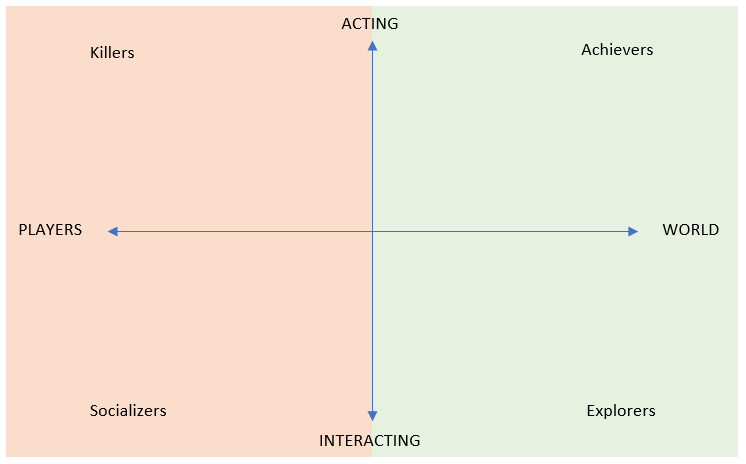
\includegraphics[width=0.75\textwidth, keepaspectratio]{Bilder/Diagramme/InterestGraphBartleAchieversExplorers.png}
	\caption{Benutzeroberfläche Fortschrittsmanagement}
	\label{img:interestGraphBartleAchiversExplorers}
\end{figure}

\par Durch den vorgesehenen Kontext der Applikation, die Studierenden während der Bearbeitung der Bachelorarbeit wegweisend zu unterstützen und zu motivieren, bietet sich somit an, Herausforderungen und die damit verbundenen Achievements in Form von kontextbezogenen fokuslenkenden Game-Design-Elementen (siehe \ref{sec:grundlagenkapitelGamification}) in die Applikation als festen Bestandteil der Motivationsstrategie zu integrieren.

\par\medskip Wie in \citep{Sailer2016}[S. 32 - 34] beschrieben wird, besitzen Achievements verschiedene Eigenschaften, welche in Bezug auf Zielstellungen, einer steuernden und in diesem Sinne auch fordernden Funktion dienen können. Eine wichtiges Kriterium bei der Wahl der Achievements als Spiel-Design Elemente ist, dass sie dem Benutzer ein nicht-kontrollierendes, positives Feedback geben und somit nicht unangenehm kontrollieren oder den ohnehin schon sehr hoch ausfallenden Druck auf die Studierenden bei der Bearbeitung der Bachelorarbeit erhöhen. Es sollte in diesem Sinne nicht aus den Augen verloren werden, dass die Applikation den Studierenden positiv unterstützen soll.

\par\medskip Im weiteren Verlauf werden den Nutzergruppen entsprechend, auf Spiel-Design-Elemente wie Bestenlisten oder anderen sozialen Motivationsmodellen verzichtet.

\par Weiterhin wird das Integrieren eines Punkte- oder Levelsystems, sowie einer Avatarfunktion nicht verfolgt. Dies dient der Absicht, dass die Applikation zwar motivierende Spiel-Design-Elemente enthalten soll, jedoch dies in einem Umfang passieren soll, der keine, an Gamification desinteressierten Benutzer, ausschließt und somit in diesem Fall weiterhin eine brauchbare Hilfestellung bieten soll.

\newpage
\subsection{Übersicht der abgeleiteten Produktfunktionen und Anforderungen} \label{sub:produktfunktionen}
\par Im folgenden Verlauf sind die, aus der Aufgabenstellung und der Anforderungsanalyse erhobenen Produktanforderungen in natürlicher Sprache vorzufinden. Diese wurden an einer Anforderungsschablone aus dem Lehrbuch der Softwaretechnik von Helmut Balzert orientiert \citep[Kapitel 19 - Natürlichsprachliche Anforderungen, Seite 481]{Balzert2010} und nach Bedarf spezifiziert:\\

\begin{enumerate} [label=\textbf{PR\arabic*}]

\item \label{prod:pZeitFortschritt} \textbf{Unterstützung bei Zeit- und Fortschrittsmanagement}
\begin{enumerate} [label=\textit{[Req1.\arabic*]}]
\item \label{anf:meilensteinVerwalten} Die Software muss dem Studierenden ermöglichen, Meilensteine zu verwalten.
\begin{enumerate} [label=\textit{[Req1.1.\arabic*]}]
\item \label{uanf:meilensteinAnlegen} Das Anlegen von Meilensteinen
\item \label{uanf:meilensteinEntfernen} Das Entfernen von Meilensteinen
\item \label{uanf:meilensteinAendern} Das Ändern von Meilensteinen
\item \label{uanf:meilensteinVerschieben} Das Verschieben von Meilensteinen
\end{enumerate}

\bigskip
\item \label{anf:arbeitspaketVerwalten} Die Software muss dem Studierenden ermöglichen, den Meilensteinen zugehörige Aufgabenpakete zu verwalten.
\begin{enumerate} [label=\textit{[Req1.2.\arabic*]}]
\item \label{uanf:arbeitspaketAnlegen} Das Anlegen von Arbeitspaketen
\item \label{uanf:arbeitspaketEntfernen} Das Entfernen von Arbeitspaketen
\item \label{uanf:arbeitspaketAendern} Das Ändern von Arbeitspaketen
\item \label{uanf:arbeitspaketVerschieben} Das Verschieben von Arbeitspaketen
\item \label{uanf:arbeitspaketMarkieren} Das Markieren von Arbeitspaketen als \textit{abgeschlossen}
\item \label{uanf:arbeitspaketPlanen} Das Planen von Arbeitspaketen
\end{enumerate}

\bigskip
\item \label{anf:erinnerungenBenachrichtigungen}Die Software soll die Studierende auf bevorstehende Meilensteine und Aufgabenpakete aufmerksam machen.

\begin{enumerate} [label=\textit{[Req1.3.\arabic*]}]
\item \label{uanf:erinnerungAusloesen}Das Auslösen von Erinnerungen/Benachrichtigungen
\end{enumerate}
\end{enumerate}

\newpage
\item \label{prod:unterstuetzungBachelorarbeit} \textbf{Unterstützung bei der Bearbeitung der Bachelorarbeit}.
\begin{enumerate} [label=\textit{[Req2.\arabic*]}]

\item \label{anf:infRahmenbedingungenFormalien} Die Software muss den Studierenden Informationen über die Rahmenbedingungen und Formalien der Bachelorarbeit an der Fachhochschule Lübeck bereitstellen können.

\bigskip
\item \label{anf:infAufbauStruktur} Die Software muss den Studierenden Hinweise und Empfehlungen zu Aufbau und Struktur von Bachelorarbeiten bereitstellen können.

\bigskip
\item \label{anf:infDurchfuerungBachelorarbeit} Die Software muss den Studierenden Hinweise und Empfehlungen zur Durchführung von Bachelorarbeiten bereitstellen können.

\bigskip
\item \label{anf:infMethodenTechniken} Die Software muss den Studierenden eine Übersicht über studiengangs-spezifischen und -übergreifenden relevante Techniken und Methoden bereitstellen können.

\begin{enumerate} [label=\textit{[Req2.4.\arabic*]}]
\item \label{uanf:infThemenfindung} Hilfestellung/Übersicht zu Themenfindung für Bachelorarbeit
\item \label{uanf:infInhalt} Hilfestellung/Übersicht von studiengangs-spezifischen Inhalten
\item \label{uanf:infAufbereitungErgebnisse} Hilfestellung/Übersicht zu Aufbereitung von Ergebnissen
\item \label{uanf:infNachweisfuerung} Hilfestellung/Übersicht zu Nachweisführung
\end{enumerate}

\bigskip
\item \label{anf:anpassungZielgruppen} Die Software muss den Umgang von zielgruppen-spezifischen Anpassungen der Inhalte ermöglichen können.

\bigskip
\item \label{anf:anpassungSoftwareextern} Die Anpassungen der Inhalte soll software-extern realisierbar und integrierbar sein.
\end{enumerate}

\item\label{prod:gamificationelementeEinsatz} \textbf{Einsatz von Gamificationelementen zur Steigerung der Motivation}
\begin{enumerate} [label=\textit{[Req3.\arabic*]}]
\item \label{anf:spielDesignElementeBenutzerklassen} Die Software muss im Rahmen der Gamificationstrategie, Spiel-Design-Elemente bereitstellen, welche der ermittelten Benutzerklassen entsprechen.

\bigskip
\item \label{anf:spielDesignElementeOrientiertungAnBachelorarabeit} Die Spiel-Design-Elemente sollen unter Berücksichtigung der wegweisenden Eigenschaft, geeignet an dem Ablauf einer Bachelorarbeit orientiert sein.
\end{enumerate}

\bigskip
\item \textbf{\label{prod:sonstige} Weitere Anforderungen}
\begin{enumerate} [label=\textit{[Req4.\arabic*]}]
\item \label{anf:mehrsprachig} Die Software muss sämtliche Inhalte und Leistungen auch für international-sprachige Personengruppen enthalten.

\bigskip
\item \label{anf:persoenlicheThemenvorschlaege} Die Software kann die Möglichkeit bieten, dass Betreuer ihre persönlichen Themenvorschläge für die Studierenden sichtbar, per Weboberfläche hinzufügen/entfernen können 
\end{enumerate}


\end{enumerate}

\newpage
\subsection{Übersicht der Risiken} \label{sub:risikouebersicht}
\par Im Laufe der mit den Professoren durchgeführten Interviews, wurden häufig Bedenken geäußert bezüglich der Risiken, die der Einsatz der Software für die Studierenden mit sich bringen könnte. 
\par \bigskip Es folgt die Aufzählung der ermittelten Risiken, sowie einer Gewichtung in Bezug auf die stärke der negativen Auswirkungen bei Eintreten dieser Risiken:

\begin{enumerate} [label=\textit{[R\arabic*]}]
\item \label{risk:realerZustand} 
\par Auswirkungen: Hoch
\par Die Applikation kennt den realen Zustand und Fortschritt der Bachelorarbeit nicht und könnte somit zu einer Verfälschung des realen Bildes führen. Studierende könnten somit den eigentlichen Zustand der Arbeit aus den Augen verlieren.
\item \label{risk:inhaltUnumstoesslich} 
\par Auswirkungen: Hoch
\par Studierende könnten die Hilfestellung der Applikation als unumstößlich ansehen und so unter Umständen in Konflikt mit dem Betreuer kommen.
\item \label{risk:erstazBetreuer} 
\par Auswirkungen: Hoch
\par Die Applikation kann als Ersatz für die Betreuung von einem Professor oder Professorin wahrgenommen werden, was zu weitreichenden Konsequenzen für die Qualität der Abschlussarbeit führen könnte.
\item \label{risk:keinLerneffekt} 
\par Auswirkungen: Hoch
\par Durch die Nutzung der Applikation wird dem Studierenden so viel Arbeit abgenommen, dass der Lerneffekt der Bachelorarbeit zu gering ist.
\item \label{risk:ueberplanung} 
\par Auswirkungen: Mittel
\par Die Applikation könnte im Rahmen des Zeitmanagement-Tools zu einer Überplanung führen, was den Studierenden von der eigentlichen Arbeit abhalten könnte.
\item \label{risk:gamificationEffekt} 
\par Auswirkungen: Gering
\par Gamification-Elemente können einen sehr geringen Effekt haben, da nicht sie die Motivation aufrecht erhalten, sondern die Interesse des Studierenden.
\end{enumerate}

\newpage
\subsection{Übersicht der Chancen} \label{sub:chancenuebersicht}
\par Aus den gewonnen Informationen, welche sich aus dem Verlauf der Interviews mit den Professoren und der schriftlichen Befragung mit den Studierenden ergeben haben, ließen sich Chancen für Betreuer und Studierende durch Einsatz der Applikation identifizieren, welche im Folgenden genannt werden.

\par \bigskip Es folgt die Aufzählung der ermittelten Chancen, sowie einer Gewichtung in Bezug auf die stärke der positiven Auswirkungen bei Erreichen dieser Chancen:

\begin{enumerate} [label=\textit{[C\arabic*]}]
\item 
\par Auswirkungen: Hoch
\par Aufnahmebereitschaft gegenüber Tipps, Empfehlungen und anderen Aspekten könnte im Gegensatz zum Bachelorarbeit-Seminar gesteigert werden, da der Einsatz der Applikation von begleitender Natur ist und sich die Studierenden somit besser mit dem Problem identifizieren könnten.
\item
\par Auswirkungen: Hoch
\par Vermeiden von großen Fehlern der Studierenden, durch Lenken des Fokus der Studierenden auf wichtige Aspekte der Bachelorarbeit, bei denen üblicherweise häufig Probleme auftreten.
\item
\par Auswirkungen: Hoch
\par Besseres Zeitmanagement der Studierenden und die Steigerung der organisatorischen Fähigkeiten durch Anwendung der Applikation.
\item
\par Auswirkungen: Hoch
\par Systematischere Vorgehensweise der Studierenden bei Problemanalyse, Anforderungserhebung und Nachweisführung
\item
\par Auswirkungen: Hoch
\par Senken des Beratungsaufwandes seitens der Betreuer bei Trivialitäten und bei sich wiederholenden Fragestellungen.
\item 
\par Auswirkungen: Mittel
\par Neuer Informationskanal für Studierende, welcher Wissenslücken bezüglich der Rahmenbedingungen und Regeln einer Bachelorarbeit schließen kann.
\item
\par Auswirkungen: Mittel
\par Zielgerichteterer Methoden- und Werkzeugeinsatz, sowie Anwendung fachspezifischer und fachübergreifender Techniken.
\item
\par Auswirkungen: Mittel
\par Minimieren von Problemen bei der Gestaltung der Dokumentation.
\item
\par Auswirkungen: Gering
\par Bessere Vorbereitung der Studierenden auf Gesprächsterminen mit dem Betreuer.
\end{enumerate}



\chapter{Konzeptvorstellung der Applikation} \label{chap:konzept}

\section{Beschreibung der Software}
\par Die Applikation ist in verschiedene Kern-Softwareabschnitten unterteilt. Diese Abschnitte lassen sich weiterhin auf folgende namensgebende Aufgabenbereiche aufteilen, welche sich an den erhobenen Anforderungen und der Aufgabenstellung orientieren (siehe Kapitel \ref{sub:produktfunktionen}).

\begin{itemize}
\item Fortschrittsmanagement
\item Guide
\item Herausforderungen
\item Achievements
\item Sonstige Softwareinhalte
\item Dashboard
\end{itemize}

\newpage
\subsection{Fortschrittsmanagement}
\par Das Fortschrittsmanagement ist ein Tool, welches das Anlegen, Planen und Verwalten von Meilensteinen, sowie der Arbeitspakete ermöglichen soll. 

\par\bigskip Es folgt eine stichpunktartige Auflistung und Beschreibung der Kernfeatures des Tools:
\begin{itemize}
\item \textbf{Ein Zeitstrahl als Grundlage}
\par Der scrollbare Zeitstrahl bietet die Arbeitsgrundlage des Fortschrittsmanagement-Tools. Hier können wochenweise Meilensteine mit Arbeitspaketen angelegt werden.  \ref{anf:meilensteinVerwalten}
\item \textbf{Erstellung und Verwaltung von Meilensteinen}
\par Es können Meilensteine erstellt \ref{uanf:meilensteinAnlegen}, bearbeitet\ref{uanf:meilensteinAendern}, verschoben\ref{uanf:meilensteinVerschieben} und entfernt\ref{uanf:meilensteinEntfernen} werden. Jeder Woche kann maximal ein Meilenstein zugeordnet werden.
\item \textbf{Erstellung und Verwaltung von Arbeitspaketen}
\par Jeder Meilenstein enthält Arbeitspakete\ref{anf:arbeitspaketVerwalten}, die von dem Benutzer einem Meilenstein hinzugefügt\ref{uanf:arbeitspaketAnlegen}, bearbeitet\ref{uanf:arbeitspaketAendern}, verschoben\ref{uanf:arbeitspaketVerschieben} und gelöscht\ref{uanf:arbeitspaketEntfernen} werden können. Weiterhin lassen sich die Arbeitspakete optional konkreten Wochen zuordnen, um eine individuelle Planung\ref{uanf:arbeitspaketPlanen} zu ermöglichen und als abgeschlossen markieren\ref{uanf:arbeitspaketMarkieren}.
\end{itemize}

\begin{figure}[H]
	\centering
	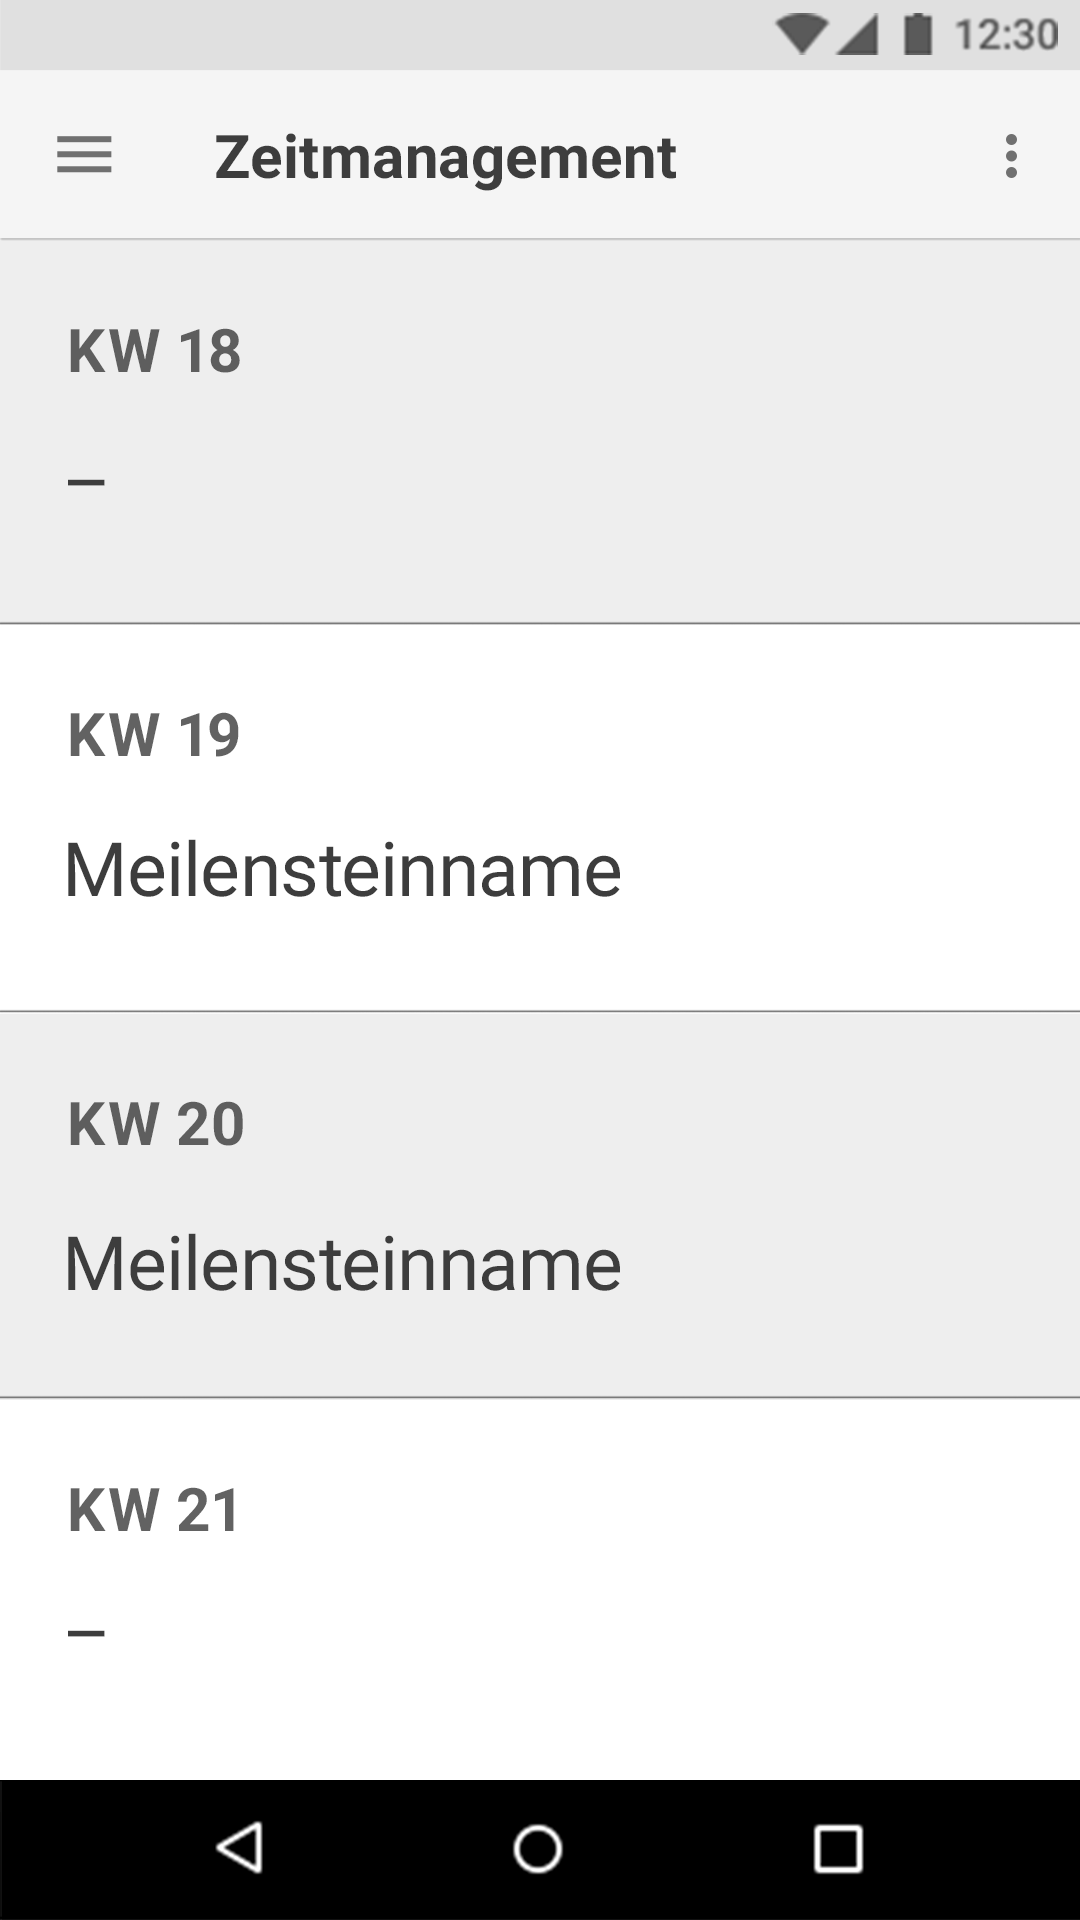
\includegraphics[width=0.35\textwidth, keepaspectratio]{Bilder/Prototyp/Zeitmanagement.png}
	\caption{Benutzeroberfläche Fortschrittsmanagement}
	\label{img:fortschrittsmanagement}
\end{figure}

\par \medskip


\newpage
\subsection{Guide}
\par Der Guide stellt den Teil der Applikation dar, der die Bereitstellung von Hinweisen, Tipps und weiteren hilfreichen Informationen zur Bearbeitung der Bachelorarbeit abdecken soll. Dieser Inhalt ergibt sich aus der Verwendung des, von der Fachhochschule Lübeck ausgehändigten Dokuments, welches als Ratgeber bei der Erstellung von Bachelorarbeiten funktionieren und somit die speziellen Anforderungen der FH-Lübeck berücksichtigen soll \citep[vgl. Kapitel 1]{FHLuebeckBAAnleitung}.
\par In dieser Hinsicht soll der Guide als genereller Anlaufpunkt funktionieren, der beispielsweise eine Hilfestellung für Bacheloranden darstellen.

\par\medskip Die Bandbreite der Hinweise, Tipps und Informationen sollen somit den gesamten Verlauf der Bachelorarbeit abdecken und lassen sich in diesem Umfang in folgende Bereiche und Inhalte Zerlegen, welche sich an dem Leitfaden der FH-Lübeck\citep{FHLuebeckBAAnleitung} zur Erstellung einer Bachelorarbeit orientieren.

\par\medskip Es folgt eine Interpretation und Beschreibung der Unterteilung der Themengebiete:

\par\medskip \textit{Anmerkung: Die folgenden Themengebiete/Softwareabschnitte stellen nur eine Möglichkeit der Aufteilung dar. Bei Einsatz der Software sollen die hier dargestellten Inhalte individuell erweitert oder verändert werden können.}

\begin{itemize}
\item \textbf{Allgemeine Informationen}
\par Dieser Abschnitt beinhaltet die allgemeinen Informationen , welche vor allem zur Klärung der Formalien bei der Bearbeitung der Abschlussarbeit wichtig sind.\ref{anf:infRahmenbedingungenFormalien}

\item \textbf{Struktur der Arbeit}
\par Der Abschnitt befasst sich näher mit dem Aufbau der Bachelorarbeit und stellt vor allem Informationen und Empfehlungen bereit, welche sich auf die Strukturierung und die Bedeutung der einzelnen Kapitel der Bachelorarbeit beziehen.\ref{anf:infAufbauStruktur}

\item \textbf{Hinweise zum Schreiben}
\par In diesem Abschnitt werden tiefgehende Informationen und Empfehlungen behandelt, welche sich auf die praktische Umsetzung des Schreibens im Detail beziehen. Beispielhaft hierfür sind der Schreibstil, die Verwendung von Zeiten oder die Einbindung von Bildern, Tabellen und Programmcode.\ref{anf:infDurchfuerungBachelorarbeit}

\item \textbf{Methodenübersicht}
\par Dieser Abschnitt bietet eine Übersicht, wichtiger Methoden der Informatik, die sich bei der Bearbeitung und Dokumentation der Bachelorarbeit als Hilfreich erweisen könnten.\ref{anf:infMethodenTechniken}

\item \textbf{FAQ}
\par Dieses Kapitel behandelt oft gestellte Fragen und verdeutlicht die Informationen in der Form eines Frage-Antwort Schemas.
\end{itemize}

\newpage
\bigskip
\begin{figure}[H]
	\subfigure[Guide Hauptbildschirm]{
\includegraphics[width=0.33\textwidth]{Bilder/Prototyp/Guide.png}}
	\subfigure[Guide Themen-Ebene]{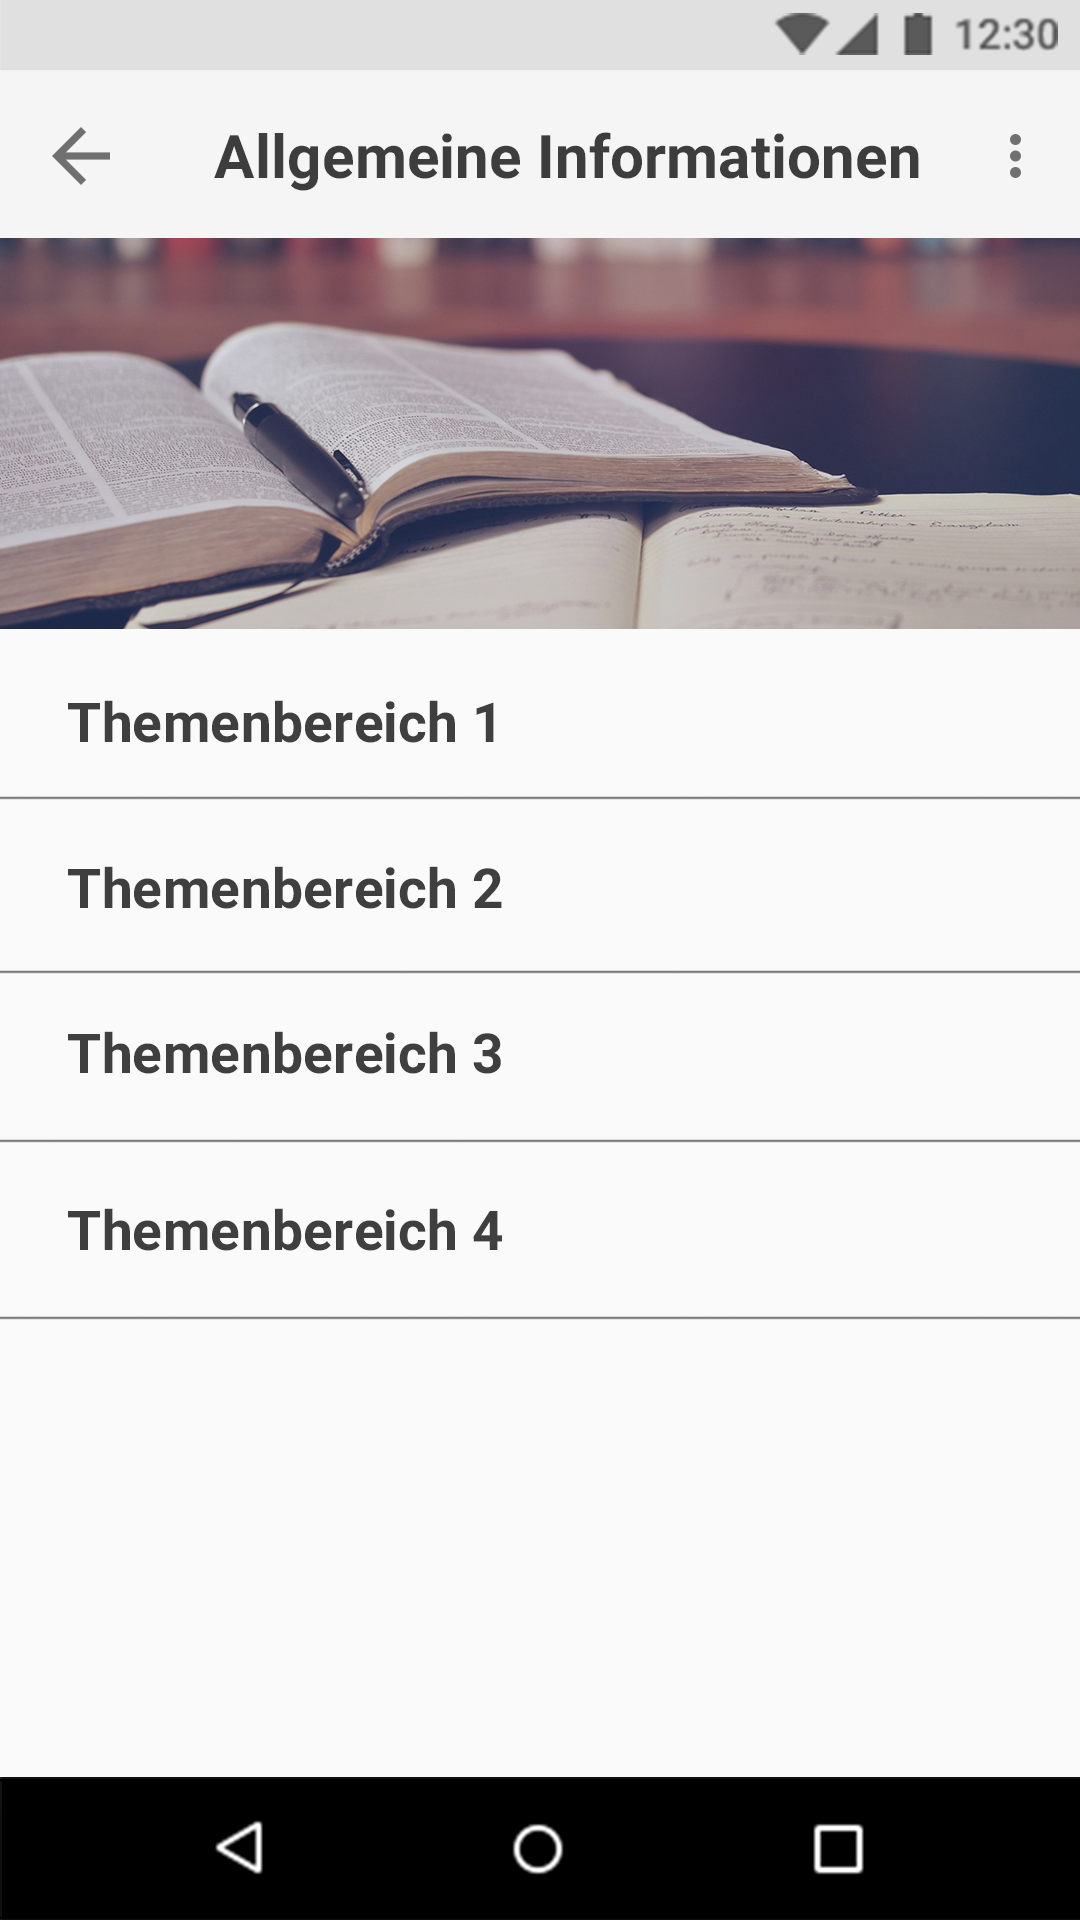
\includegraphics[width=0.33\textwidth]{Bilder/Prototyp/GuideThemenbereich.png}}
	\subfigure[Guide Informations-Ebene]{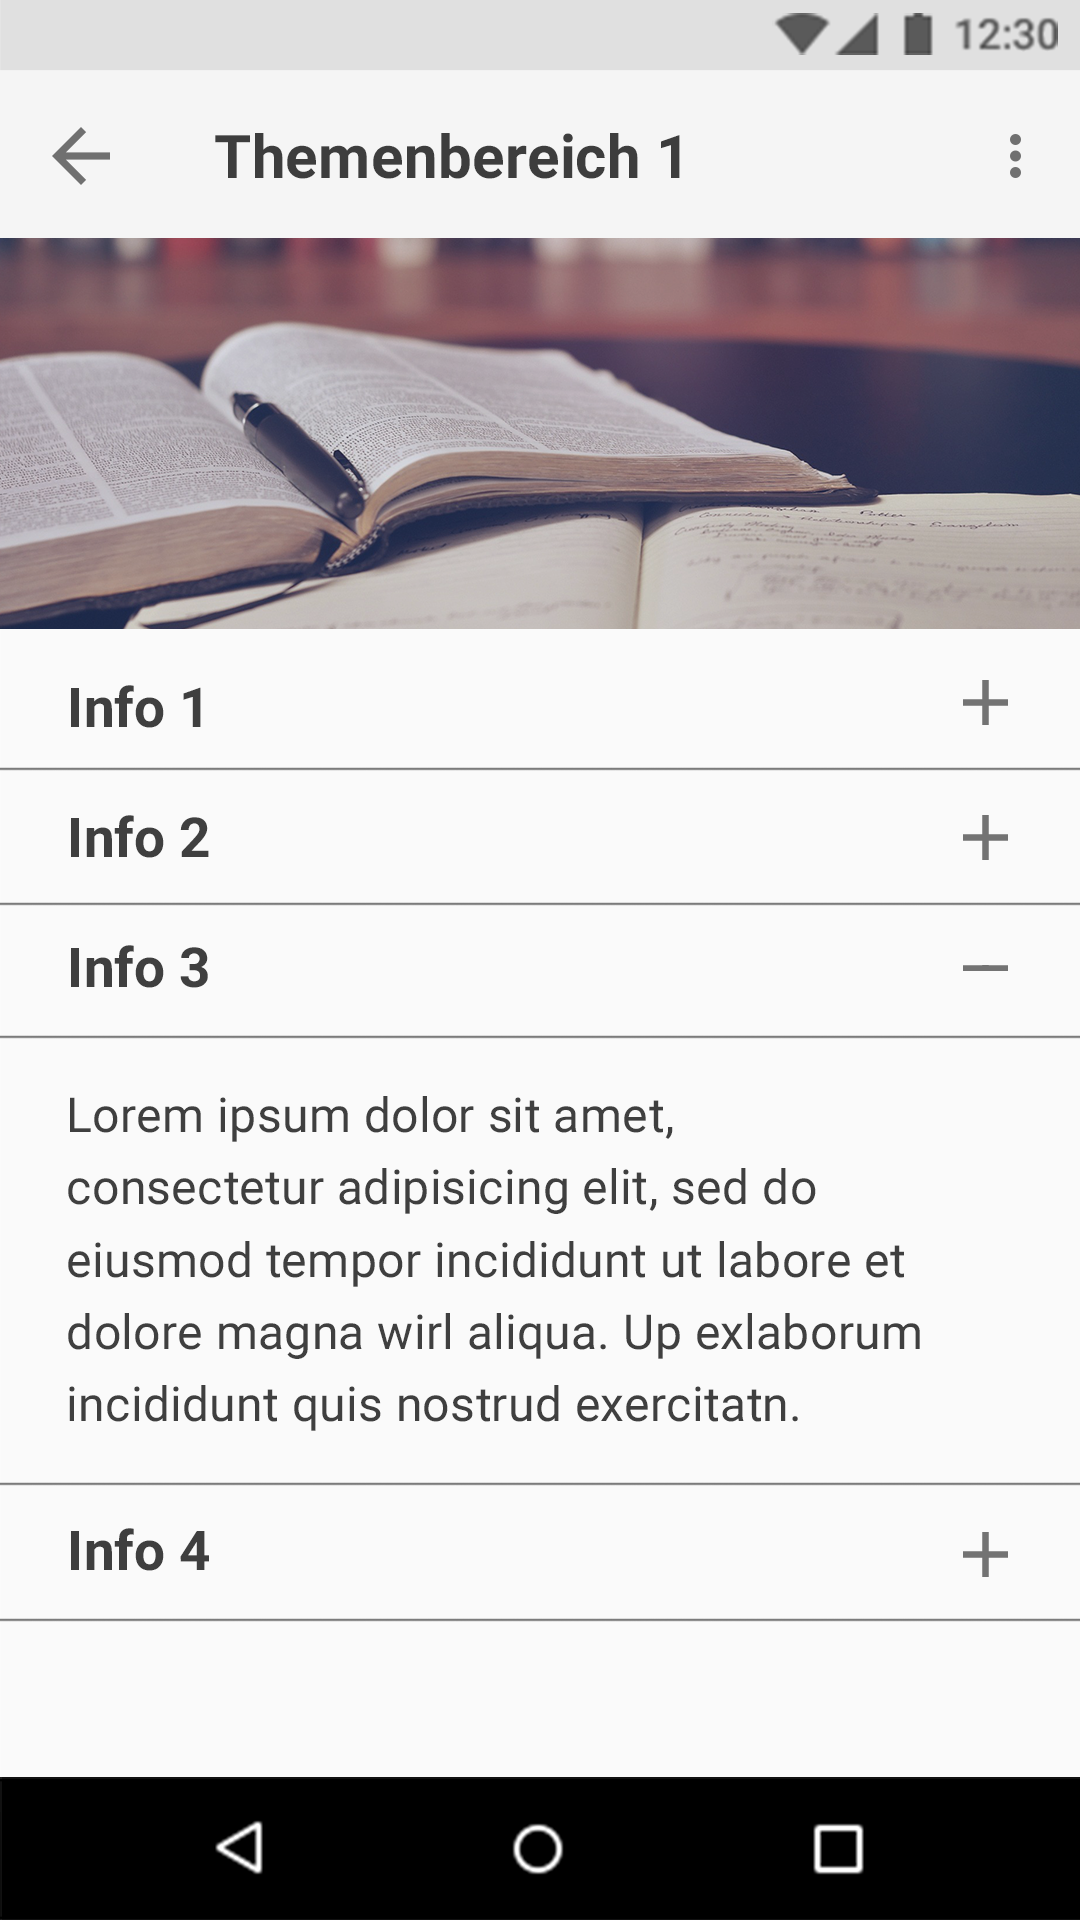
\includegraphics[width=0.33\textwidth]{Bilder/Prototyp/GuideThemenbereichInformationen.png}}
	\caption{Benutzeroberfläche Guide}
	\label{img:guide}
\end{figure}

\newpage
\subsection{Herausforderungen}
\par In diesem Bereich der Applikation kann der Benutzer einsehen, welche Herausforderungen \ref{anf:spielDesignElementeBenutzerklassen} schon abgeschlossen wurden und welche noch offen sind. Die Herausforderungen sind nach festgelegten Kategorien geordnet und orientieren sich nach dem typischen Ablauf einer Bachelorarbeit\ref{anf:spielDesignElementeOrientiertungAnBachelorarabeit}. Bei öffnen der Kategorien, gelangt der Benutzer in eine tiefere Ebene, in der die jeweiligen, noch zu erledigen oder abgeschlossenen Herausforderungen, einzusehen sind.

\begin{figure}[H]
	\centering
	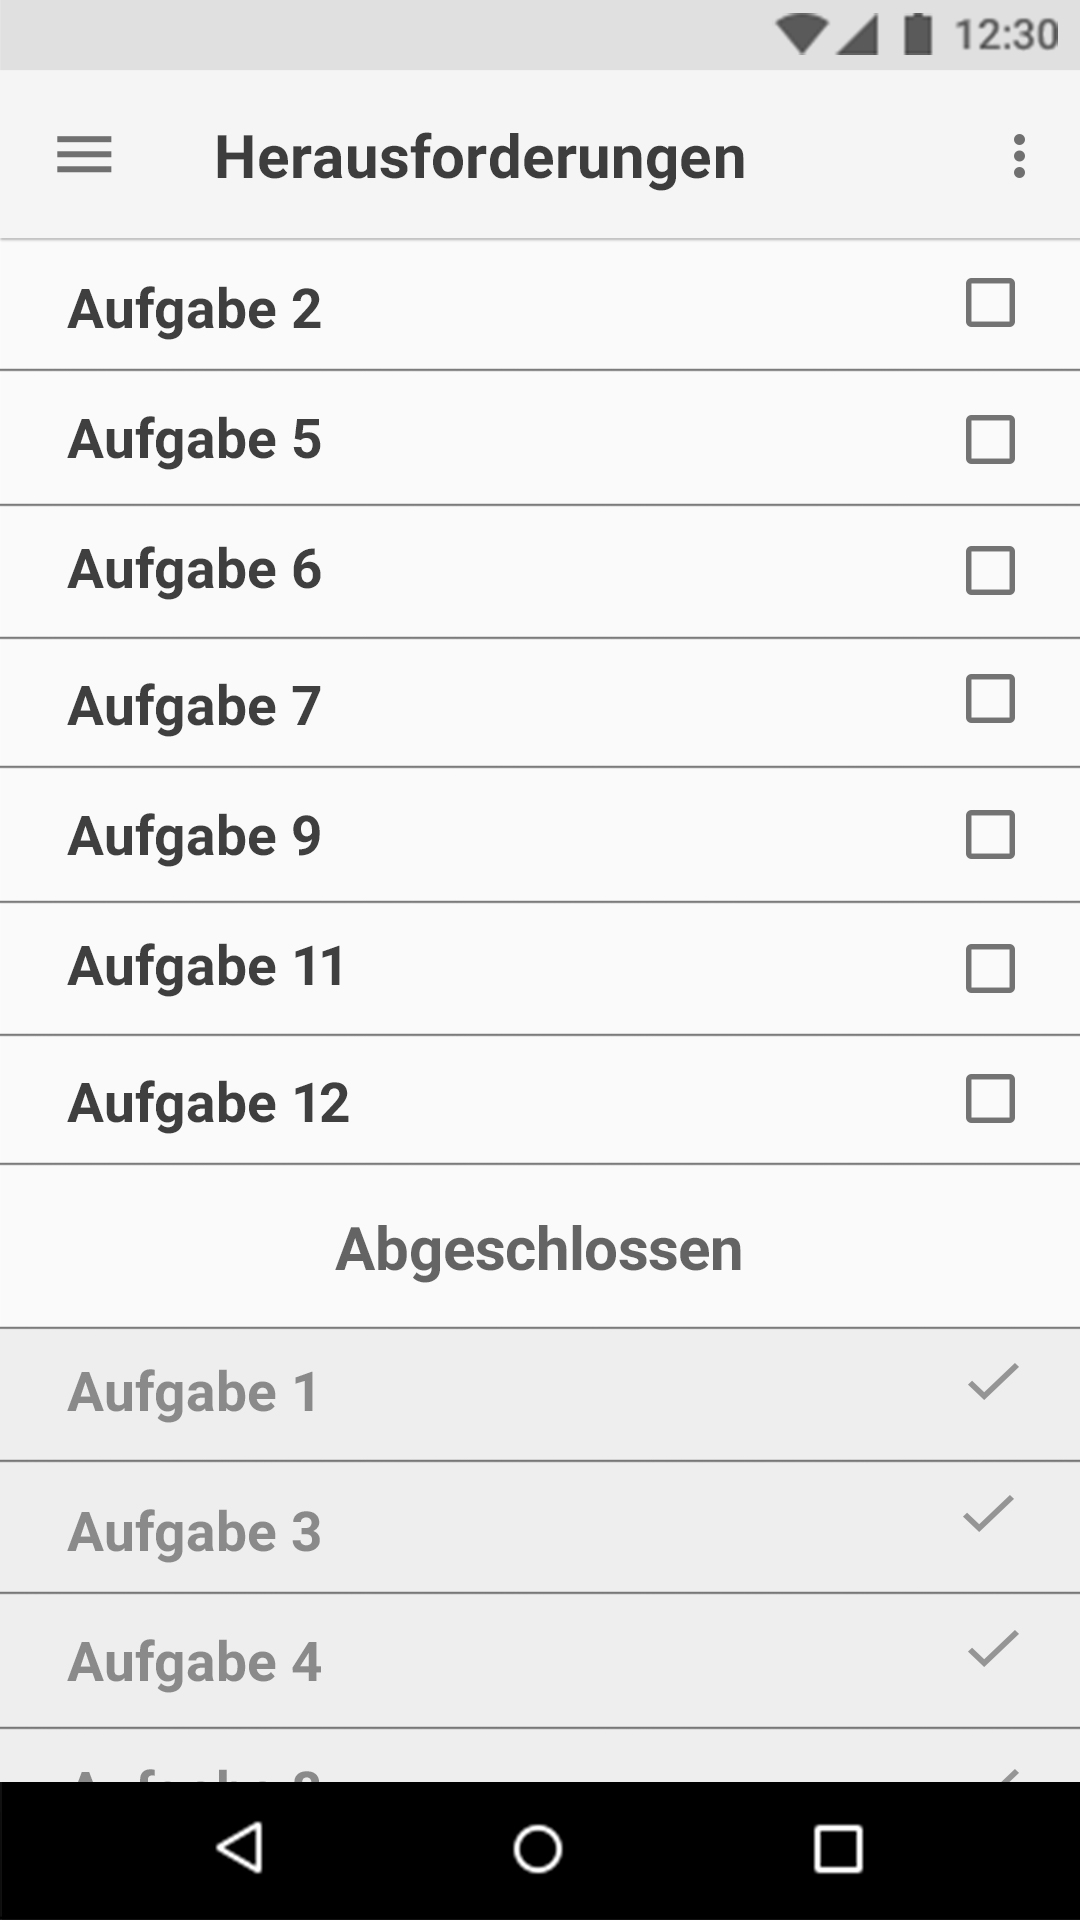
\includegraphics[width=0.4\textwidth, keepaspectratio]{Bilder/Prototyp/AufgabenSortiert.jpg}
	\caption{Benutzeroberfläche Herausforderungen}
	\label{img:aufgaben}
\end{figure}

\newpage
\subsection{Achievements}
\par Der Achievement-Hauptbildschirm\ref{anf:spielDesignElementeBenutzerklassen} enthält eine Übersicht der verschiedenen Kategorien von Achievements (siehe Abbildung \ref{img:achievements}). Die nächste Ebene dieses Abschnitts zeigt die detaillierte Ansicht der jeweiligen Achievements an, wo sich der Benutzer einsehen kann, welche Achievements er bereits erhalten hat. Weitere Informationen zu den einzelnen Achievement und deren Kategorien finden ich im Kapitel \ref{sec:gamificationelemente}\\

\begin{figure}[H]
\centering
	\subfigure[Achievements Hauptbildschirm]{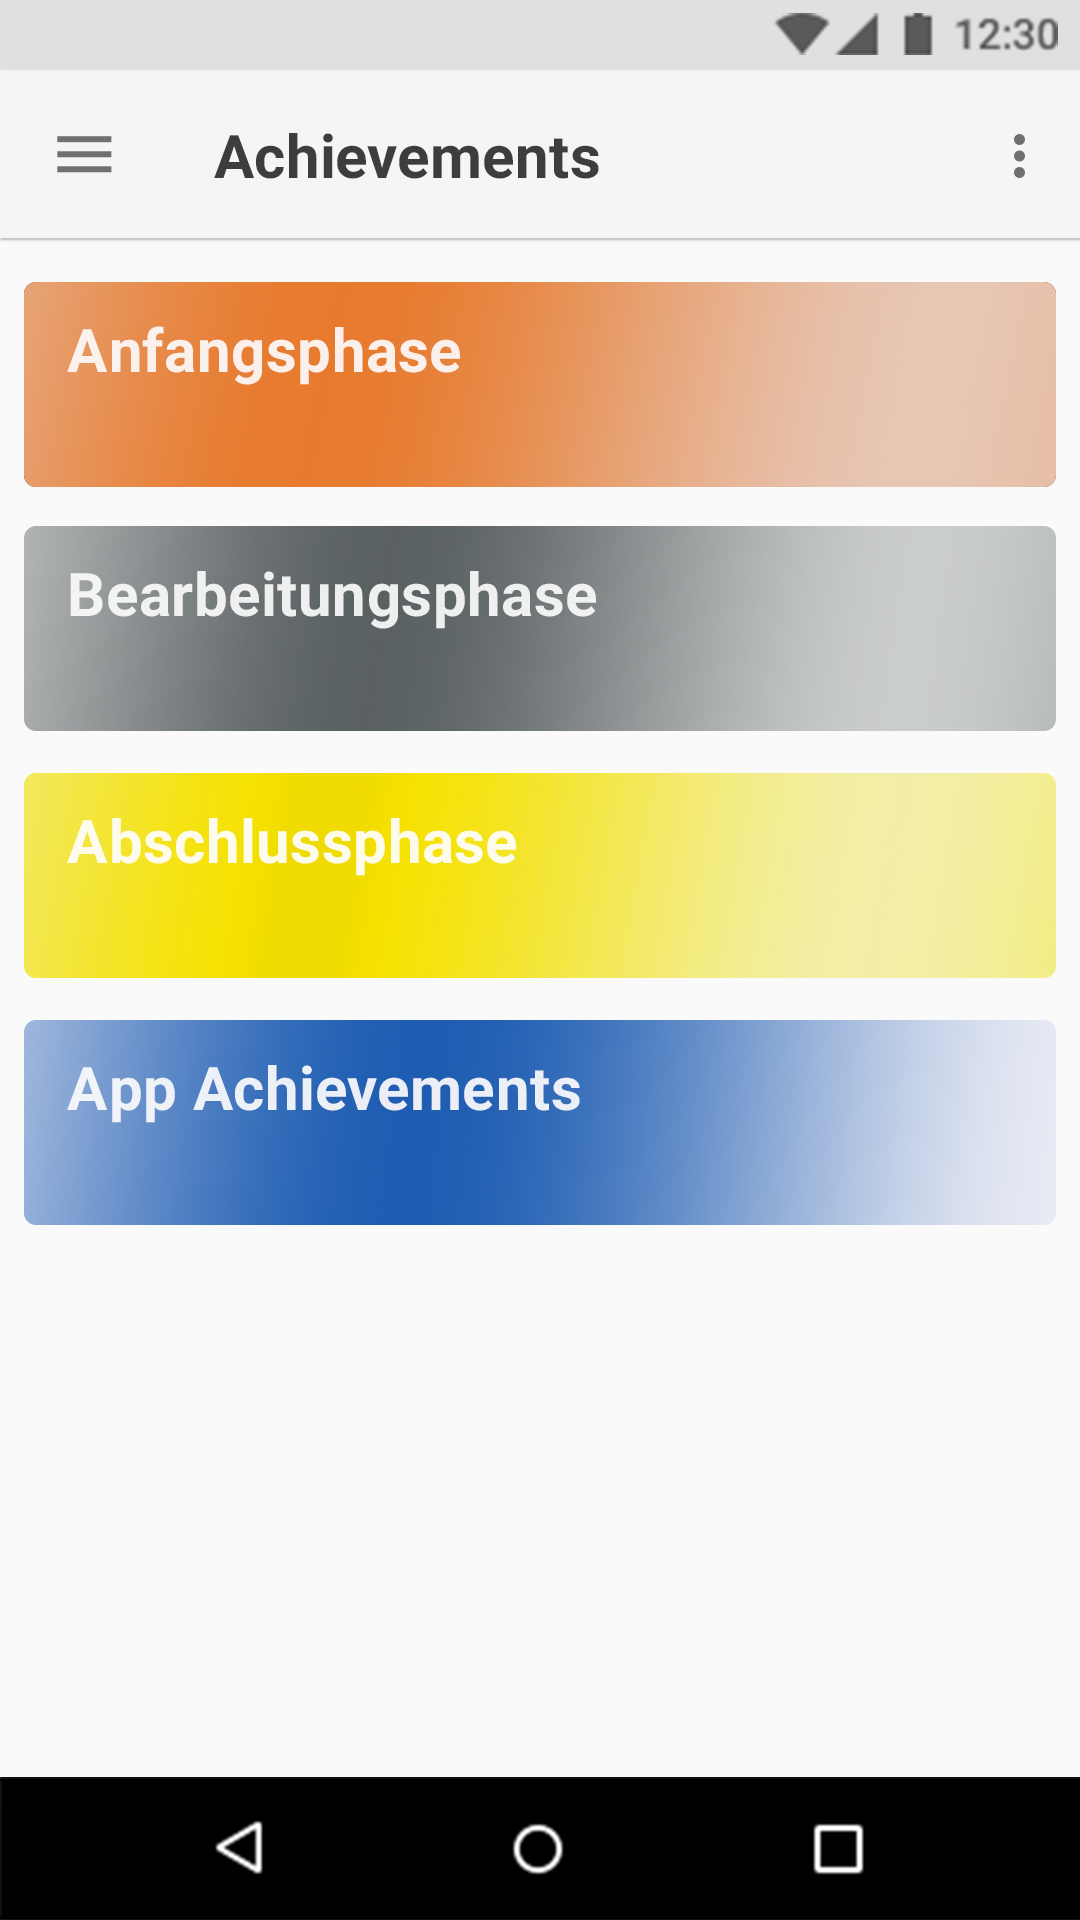
\includegraphics[width=0.35\textwidth]{Bilder/Prototyp/AchievementsUebersicht}}
	\subfigure[Achievements]{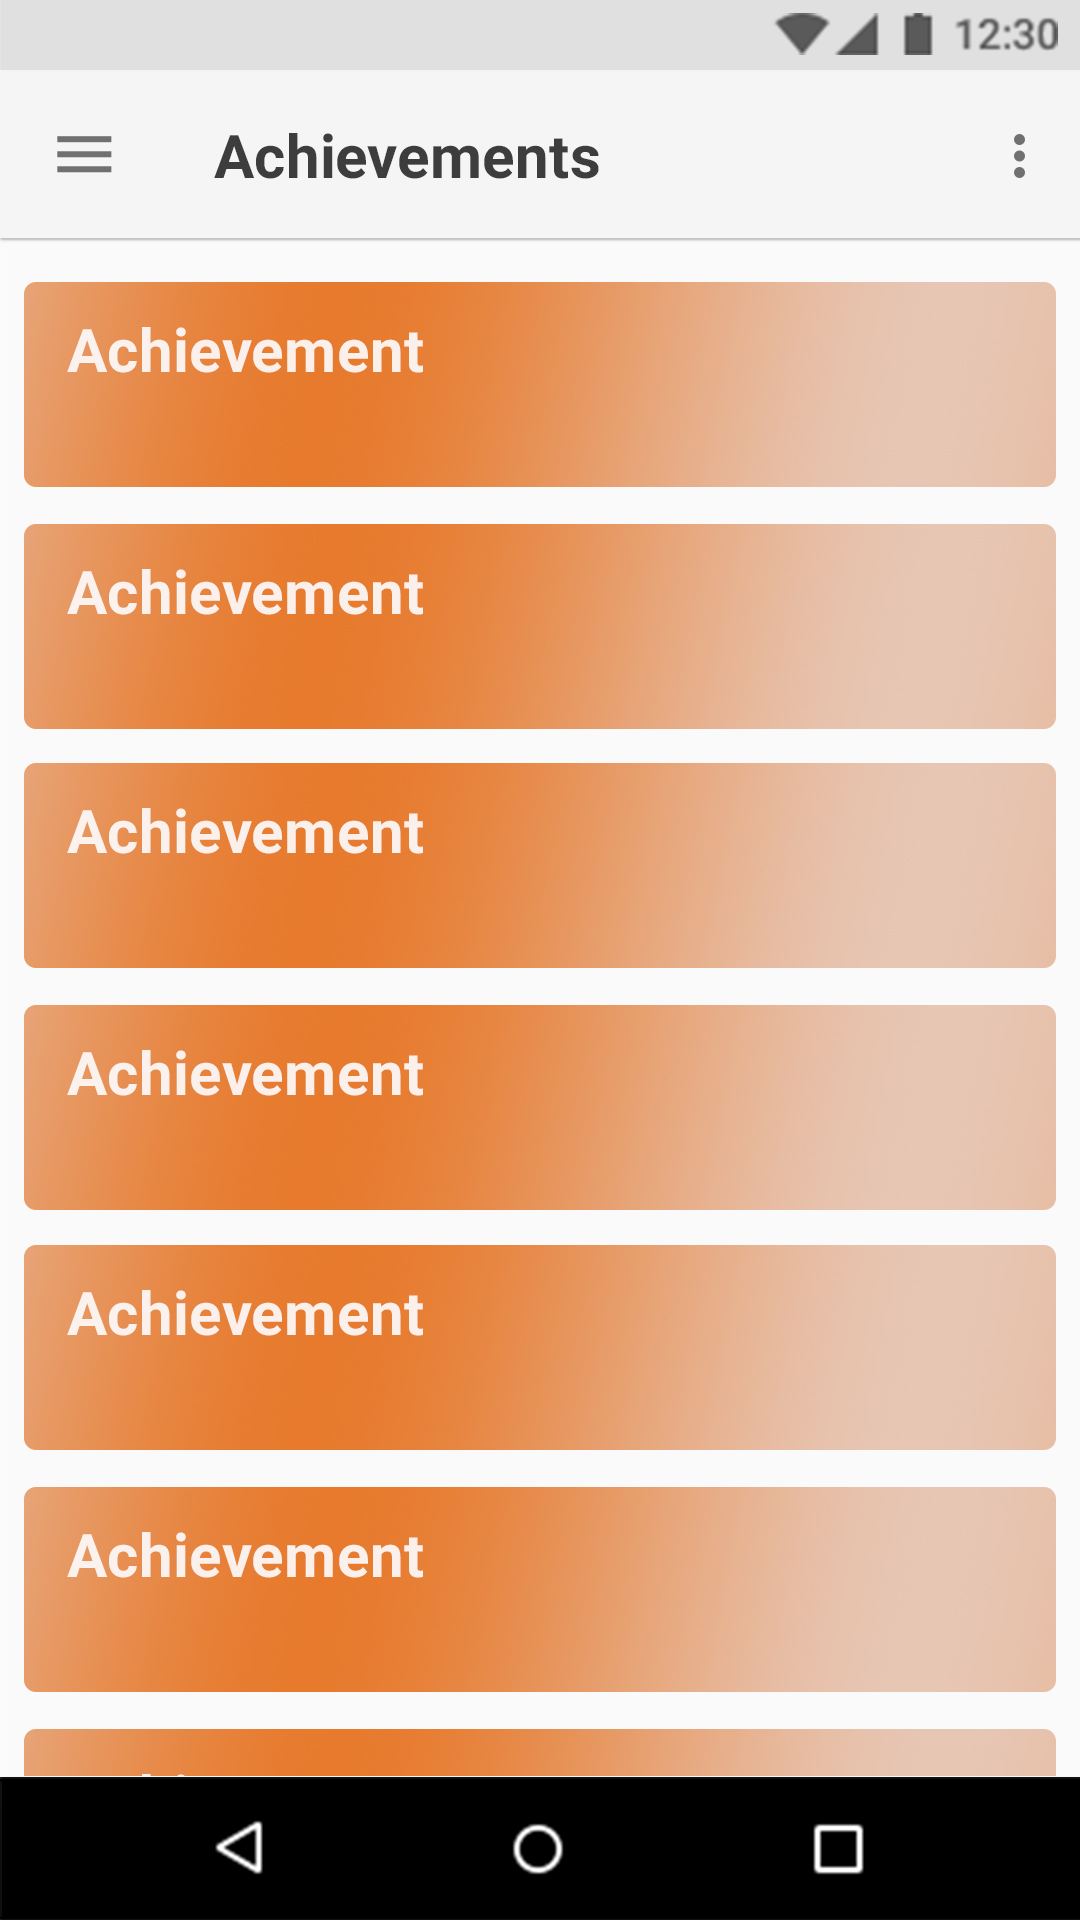
\includegraphics[width=0.35\textwidth]{Bilder/Prototyp/AchievementsUebersichtAchievements.jpg}}
	\caption{Benutzeroberfläche Achievements}
	\label{img:achievements}
\end{figure}

\newpage
\subsection{Sonstige Softwareinhalte}
\par Über die eigentlichen individuellen Funktionalitäten hinaus, sind weitere Grundfunktionalitäten vorhanden, welche unter den Punkt \textbf{Sonstige Softwareinhalte} fallen.

\par\medskip Es folgt eine stichpunktartige Auflistung und Beschreibung der Inhalte:
\begin{itemize}
\item \textbf{Menü}
\par Das Menü zeigt die existierenden Funktionalitäten und Softwareabschnitte in einer klassischen gelisteten Menüstruktur.
\item \textbf{Einstellungen}
\par Die Einstellungen beinhalten Optionen, die sich auf die Eigenschaften der Applikation auswirken. Beispielsweise das Verändern des Designs oder der Sprache\ref{anf:mehrsprachig}
\end{itemize}

\begin{figure}[H]
	\centering
	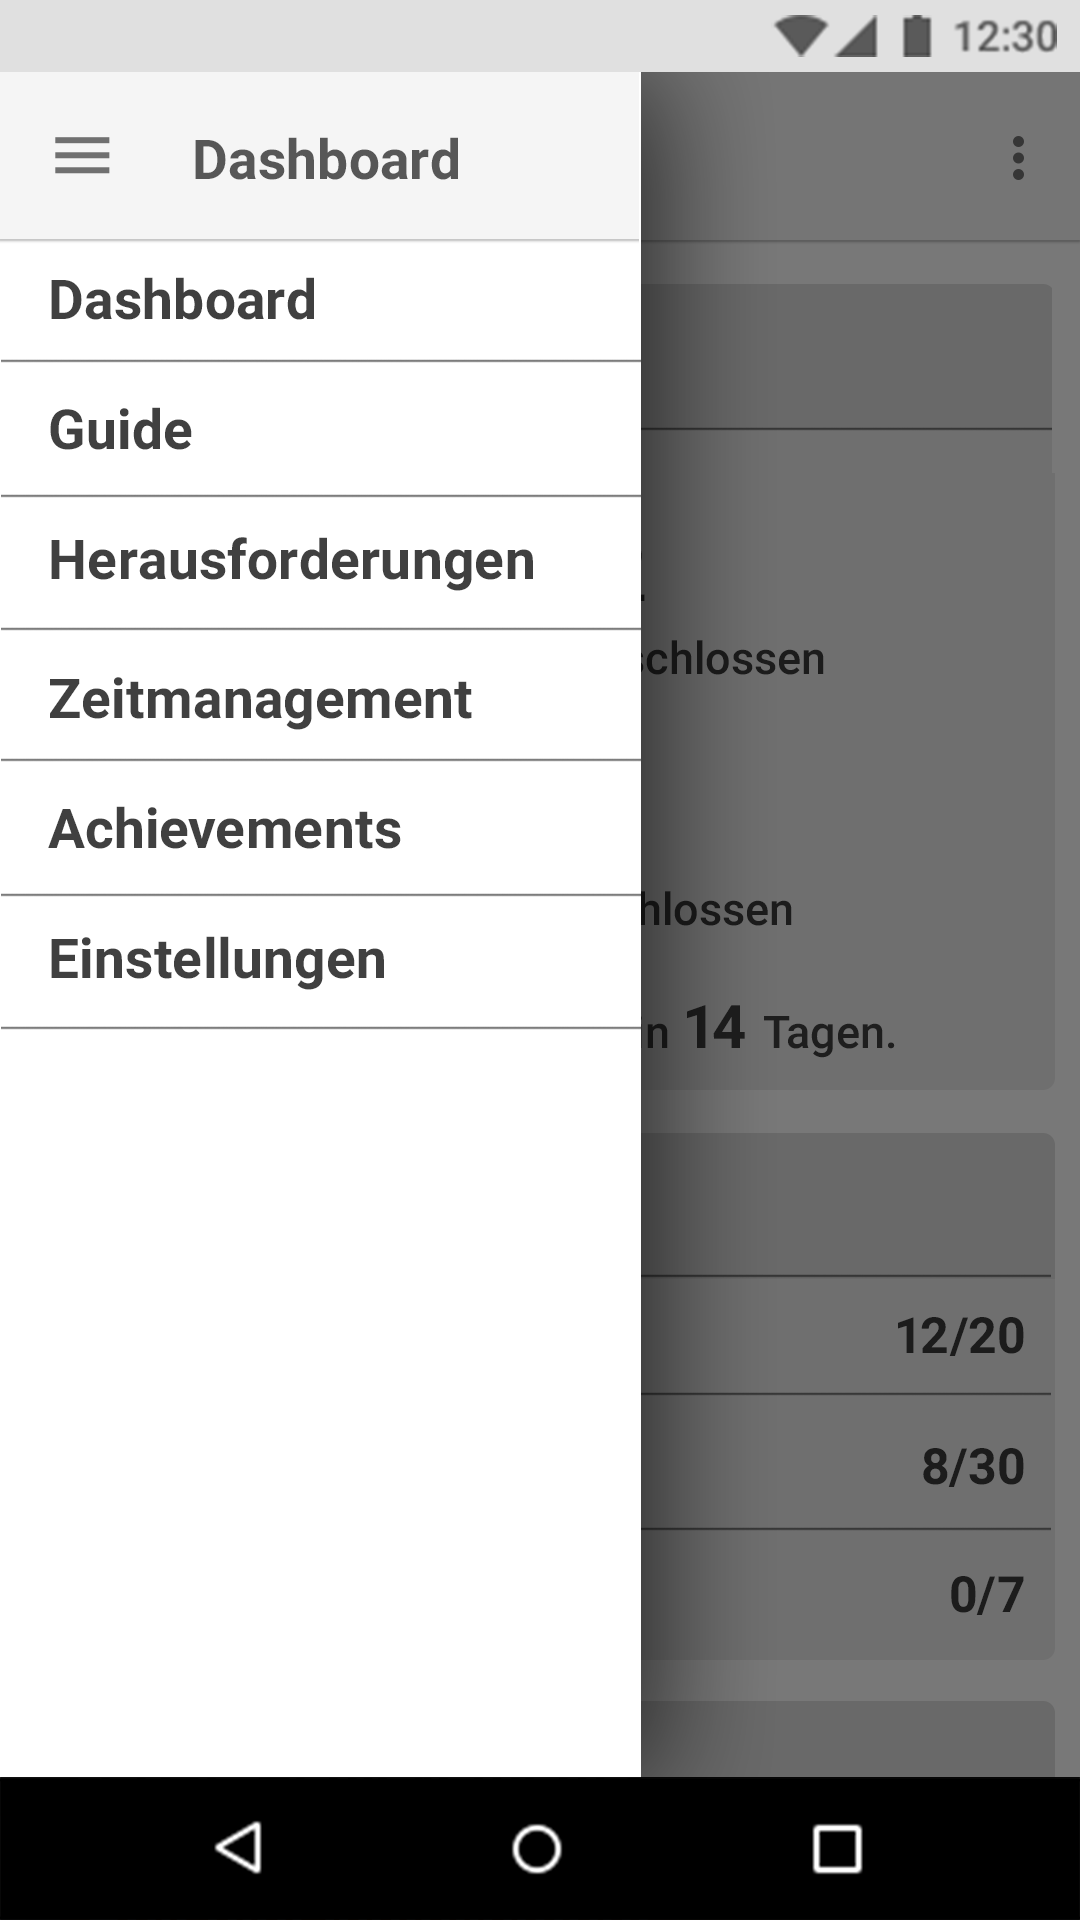
\includegraphics[width=0.4\textwidth,keepaspectratio]{Bilder/Prototyp/Menu.png}
	\caption{Benutzeroberfläche Navigations-Menü}
	\label{img:navigation}
\end{figure}

\newpage
\subsection{Dashboard}
\par Das Dashboard stellt den Ausgangspunkt und Hauptbildschirm der Applikation dar und trägt somit die Aufgabe, aktuelle Informationen für den Nutzer aufbereitet anzuzeigen, sowie die Funktionen der Applikation auf einfache Weise zugänglich zu machen. Von diesem Punkt aus soll der Benutzer die verschiedenen Softwareabschnitte öffnen können, weshalb es eine essenzielle Eigenschaft des Dashboards ist, die Inhalte übersichtlich, strukturiert und gleichzeitig aber visuell ansprechend darzustellen.

\par \medskip Es folgt eine stichpunktartige Auflistung und Beschreibung der Inhalte:
\begin{itemize}
\item \textbf{Dynamische Anzeige des Fortschritts}
\par Der bisher geleistete Gesamtfortschritt wird verdeutlicht, indem zu sehen ist, wie viele Meilensteine in Relation zu den Gesamtmeilenstein bisher abschlossen wurden. Weiterhin wird der bisher geleistete Wochenfortschritt verdeutlicht, indem zu sehen ist, wie viele Aufgabenpakete in der Phase bis zum nächsten Meilenstein, in Relation zu den vorher definierten gesamten Arbeitspaketen, schon erfüllt wurden.
\item \textbf{Anzeige der noch offenen Herausforderungen}
\par Es wird angezeigt, wievielte Herausforderungen der jeweiligen Kategorien abgeschlossen wurden, in Relation zu deren Gesamtanzahl.
\item \textbf{Dynamische Anzeige der letzten erreichten Achievements}
\par Die Anzeige zeigt die letzten n erreichten Achievements an. Zugehörig sind in diesem Fall die Darstellung des Typs des Achievements in Form der jeweiligen Färbung, sowie den Titel der Herausforderung. Das zuletzt erreichte Achievement wird hierbei durch Größe der Darstellung und Beschreibung hervorgehoben.
\item \textbf{Dynamische Anzeige von allgemeinen Tipps}
\par Die Anzeige zeigt zufällig ausgewählte allgemeine Tipps zur Bearbeitung der Bachelorarbeit. Die Tipps wechseln nach einem definierten Zeitintervall.
\end{itemize}

\begin{figure}[H]
	\centering
	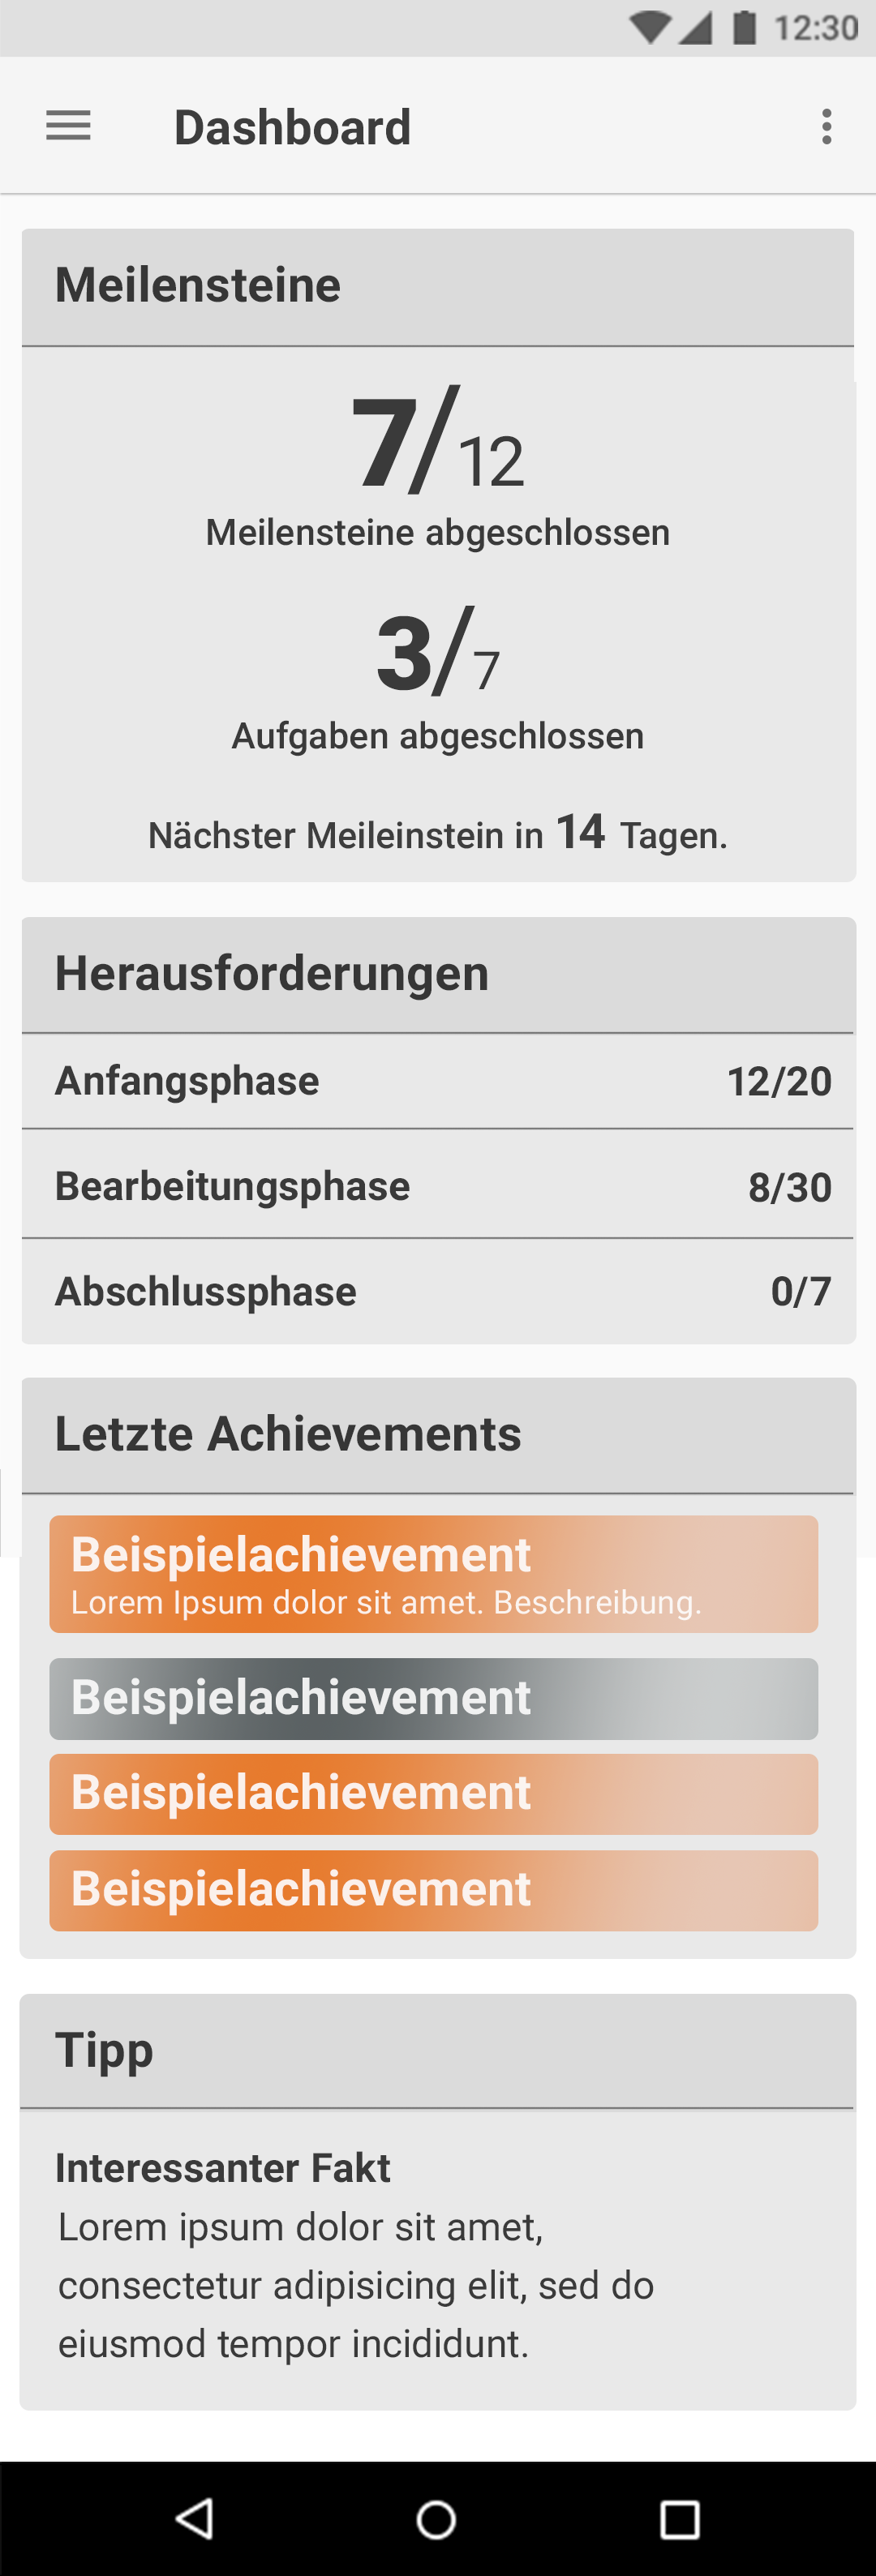
\includegraphics[width=0.45\textwidth,keepaspectratio]{Bilder/Prototyp/Dashboard.png}
	\caption{Benutzeroberfläche Dashboard}
	\label{img:dashboard}
\end{figure}


\newpage
\subsection{Übersicht der Abdeckung der Produktfunktionen}
\par Die unterschiedlichen Abschnitte der Software stehen unterschiedlich stark in Verbindung mit den verschiedenen definierten Produktanforderungen. Um eine Übersicht über die groben Zusammenhänge zu ermöglichen, folgt eine zusammenfassende Tabelle (Siehe Tabelle \ref{tab:abdeckungProduktfunktionen}).
\bigskip

\begin{tabularx}{\textwidth}{l|X|c|c|c|c|c|c}
\toprule
\textbf{Bezeichnung} 
& \textbf{Beschreibung} 
& \textbf{A1} 
& \textbf{A2} 
& \textbf{A3} 
& \textbf{A4} 
& \textbf{A5} 
& \textbf{A6}
\\ \midrule
	
\textbf{\ref{anf:meilensteinVerwalten}}
&  (Verwaltung von Meilensteinen) 
& \ding{108} 
&  
&  
&  
&  
&  
\\ \midrule
	
\textbf{\ref{anf:arbeitspaketVerwalten}}
& (Verwaltung von Aufgabenpaketen) 
& \ding{108} 
&  
&  
&  
&  
&  
\\ \midrule
	
\textbf{\ref{anf:erinnerungenBenachrichtigungen}}
& (Erinnerung an Meilensteine) 
& \ding{108} 
&  
&  
&  
&  
&  
\\ \midrule
	
\textbf{\ref{anf:infRahmenbedingungenFormalien}}
& (Hinweise zu Rahmenbedingungen und Formalien) 
&  
& \ding{108} 
&  
&  
&  
&  
\\ \midrule
	
\textbf{\ref{anf:infAufbauStruktur}}
& (Hinweise zu Aufbau und Struktur) 
&  
& \ding{108} 
&  
&  
&  
&  
\\ \midrule
	
\textbf{\ref{anf:infDurchfuerungBachelorarbeit}}
& (Hinweise zu Durchführung) 
&  
& \ding{108} 
&  
&  
&  
&  
\\ \midrule
	
\textbf{\ref{anf:infMethodenTechniken}}
& (Übersicht von Methoden und Techniken) 
&  
& \ding{108} 
&  
& 
&  
&  
\\ \midrule
	
\textbf{\ref{anf:anpassungZielgruppen}}
& (Anpassbarkeit an Zielgruppe) 
&  
& \ding{108} 
&  
&  
&  
&  
\\ \midrule
	
\textbf{\ref{anf:anpassungSoftwareextern}}
& (Software-externe Anpassung) 
&  
& \ding{108} 
&  
&  
&  
&  \\ \midrule
	
\textbf{\ref{anf:spielDesignElementeBenutzerklassen}}
& (Benutzerklassen-orientierte Spiel-Design-Elemente) 
&  
&  
& \ding{108} 
& \ding{108} 
& \ding{108} 
&  
\\ \midrule
	
\textbf{\ref{anf:spielDesignElementeOrientiertungAnBachelorarabeit}}
& (Spiel-Design-Elemente sinnvoll an Bachelorarbeit orientieren) 
&  
&  
& \ding{108} 
& \ding{108} 
&  
&  
\\ \midrule
	
\textbf{\ref{anf:mehrsprachig}}
& (Mehrsprachigkeit) 
&  
&  
&  
&  
&  
& \ding{108} 
\\ \midrule
	
\textbf{\ref{anf:persoenlicheThemenvorschlaege}}
& (Bachelorarbeitsthemen über Applikation ausschreiben)
&   
&   
&   
&  
&  
& \ding{109} 
\\ \midrule
\bottomrule
\end{tabularx}
\begin{tablenotes}
\item  A1 - Fortschrittsmanagement
\item  A2 - Guide
\item  A3 - Herausforderungen
\item  A4 - Achievements
\item  A5 - Dashboard
\item  A6 - Sonstige Softwareinhalte
\item \ding{108} - Teil der Applikation
\item \ding{109} - Als Erweiterung vorgesehen
\end{tablenotes} 
\captionof{table}{Abdeckung der Produktfunktionen}
\label{tab:abdeckungProduktfunktionen}

\newpage
\subsection{Umgang mit Risiken}
\par Im folgenden Verlauf wird der Umgang den, in Kapitel \ref{sub:risikouebersicht} dargestellten Risiken, diskutiert und beschrieben.
\par \medskip Da sich die Herausforderungen an dem Ablauf einer Bachelorarbeit orientieren und den Studierenden somit vor typische Aufgaben stellt, kam es im Verlauf der Interviews zu den Befürchtungen \ref{risk:realerZustand}, dass die Applikation nicht den realen Zustand der Bachelorarbeit kennt und somit der Studierende durch das Erfüllen von Herausforderungen ein Gefühl von Erfolg hat, obwohl diese Herausforderungen nicht den geforderten Qualitäten entsprechen und der Studierende dies durch das positive Feedback nicht merkt.
\par Um diesem Risiko entgegenzuwirken, sollen die erstellten Herausforderungen möglichst auffordernder Natur entsprechen (Beispiel: Beginne deine Einleitung). Bei Einsatz von Herausforderungen, welche auf inhaltliche Aspekte abzielen, sollen Checklisten zum Abschließen der Herausforderungen genutzt werden, um den Fokus auf eine allgemeingültige Vorgehensweise zu reduzieren, für die die Studierenden im Detail jedoch selbst verantwortlich sind. Auch hier wird eine klare Kommunikation durch die Applikation als zwingend erforderlich angesehen.

\par \medskip Die Befürchtung \ref{risk:keinLerneffekt}, dass die Applikation den Studierenden so viel Arbeit abnimmt, dass sie zu wenig eigenständige Erfahrung sammeln und somit der Lerneffekt zu gering ist, wird berücksichtigt, indem die Applikation einen eher informierenden Charakter aufweist, und keine Funktionalität bezüglich dem Liefern von Ergebnissen vorsieht.

\par \medskip Die Gefahren der Risiken \ref{risk:inhaltUnumstoesslich} und \ref{risk:erstazBetreuer}, welche sich damit auseinander setzen, dass die Applikation fälschlicherweise als Ersatz eines Betreuers wahrgenommen oder der Inhalt der Applikation als unumstößlich angesehen werden könnte, soll durch eine klare Kommunikation mit den Anwendern reduziert werden. Es werden als Maßnahmen einerseits immer die Quellen der Informationen angegeben und weiterhin eine allgemein sichtbare Erklärung zur Anwendung, sowie Fehlanwendung der Applikation deutlich kommuniziert.

\par \medskip  Das identifizierte Risiko \ref{risk:ueberplanung}, welches die Befürchtung einer Überplanung der Studierenden beinhaltet, was die Auswirkung haben kann, dass die Studierenden von der eigentlichen Arbeit abgehalten werden, wird als nicht ausschlaggebend betrachtet.
Studierende die zur Überplanung neigen, würden diese auch ohne Applikation durchführen. 
\par Wichtiger wird in dieser Hinsicht die Freiheit der einzelnen Planungs-Bedürfnisse durch die individuellen Studierenden angesehen, weshalb keine weiteren Maßnahmen zur Reduzierung der Planungsfreiheit getroffen werden. Weiterhin steht die Intensität der Planung nicht in der Verantwortung der Applikation, sondern in der Verantwortung der Benutzer. 

\par \medskip Das Risiko \ref{risk:gamificationEffekt}, welches sich mit dem Nichtwirken der Gamificationmotivation beschäftigt, wird als nicht weitreichend betrachtet, da die Gamificationinhalte zwar Bestandteil der Applikation, jedoch nicht zwangsweise notwendig zur Benutzung der Applikation sind. Die Spiel-Design-Elemente sollen nicht die Interesse an einem bestimmten Thema steigern, sondern dienen im Kontext der Bachelorarbeit einer wegweisenden Natur, welche motivierende Einflüsse auf die Bearbeitenden hervorrufen können, jedoch nicht müssen, um ihren Nutzen zu erfüllen. 


\newpage
\section{Beschreibung der Gamification-Elemente} \label{sec:gamificationelemente}
\par Im folgenden Kapitel werden die Gamification-Elemente, welche in der Applikation zum Einsatz kommen, näher beschrieben. Dabei wird vor allem auf die identifizierten Kategorien der Achievements eingegangen, welche den Kern der gewählten Motivationsstrategie bilden. Darüber Hinaus wird auch beschrieben, in welcher Form die gewählte Motivationsstrategie in der Realität, in Bezug auf den Fortschritt bei der Bearbeitung der Bachelorarbeit funktioniert.

\subsection{Achievements} \label{sub:konzeptGamificationAchievements}
\par Die Achievements verfolgen im Rahmen der Applikation die Aufgabe, motivierende Inhalte, vor allem für die identifizierten Benutzergruppen der \textbf{Achiever} und \textbf{Explorer} (siehe \ref{sub:nutzergruppenBartle}), zu bieten. Dies soll erreicht werden, indem die Achievements dem Benutzer als Belohnung für eine abgeschlossene Herausforderung, als Sammelstück hinzugefügt werden.
\par \medskip Im Rahmen dieser Motivationsstrategie werden verschiedenen Arten von Achievements in die Applikation integriert. Dies passiert unter anderem mit dem Ziel, eine an den Ablauf einer Bachelorarbeit gekoppelten Abstufung von Fortschritt und Erfolgen zu ermöglichen. 
\par Weiterhin werden auch die sogenannten \textit{App-Achievements} Einzug in die Applikation bekommen. Diese sollen weitestgehend die Bedürfnisse der Benutzergruppe \textbf{Explorer} ansprechen und im Gegensatz zu den anderen Achievements nicht sichtbar an eine Aufgabe gekoppelt sein, sondern im Laufe der Nutzung der Applikation durch \textit{versteckte Aufgaben} freigeschaltet und offengelegt werden können.

\par \medskip Um den Achievements, über das Sammeln und der Vervollständigung hinaus, eine Wertigkeit zu geben, werden diese durch verschiedene Farben/Texturen dargestellt. 

\par \bigskip Übersicht und Beschreibung der verschiedenen Achievement-Typen:
\begin{itemize}
\item \textbf{Initialphase-Achievements} (Rostiges Eisen)
\par Beinhaltete Achievements, welche mit den Herausforderungen gekoppelt sind, die vor Beginn der Bachelorarbeit erfolgen.
\item \textbf{Anfangsphase-Achievements} (Bronze)
\par Beinhaltete Achievements, welche mit den Herausforderungen gekoppelt sind, die nach Beginn der Bachelorarbeit erfolgen, sich noch nicht mit den einzelnen inhaltlichen Schritte der Bachelorarbeit auseinandersetzen.
\item \textbf{Bearbeitungsphase-Achievements} (Silber)
\par Beinhaltete Achievements, welche mit den Herausforderungen gekoppelt sind, die nach Beginn der Bachelorarbeit erfolgen und sich mit der eigentlichen Bearbeitung der Bachelorarbeit auseinandersetzen.
\item \textbf{Abschlussphase-Achievements} (Gold)
\par Beinhaltete Achievements, welche mit den Herausforderungen gekoppelt sind, die sich hauptsächlich mit der Abschlussphase einer Bachelorarbeit beschäftigen.
\item \textbf{App-Achievements} (Smaragd)
\par Beinhaltete Achievements, welche mit keinen offensichtlichen Herausforderungen gekoppelt sind, sondern nur durch Benutzung der Applikation erhalten werden können.
\end{itemize} 

\chapter{Architektur der Software} \label{chap:architektur}
\section{Architekturbeschreibung}
\section{Entwurfsentscheidungen}
\section{Erweiterbarkeit der Software für andere Studiengänge}
\chapter{Implementierung} \label{chap:implementierung}
\section{Umsetzung der Anforderungen}

\chapter{Validierung und Verifikation} \label{chap:nachweisführung}
\section{Abdeckung der Softwareanforderungen}
\section{Ausführung der Usabilityevaluation}

\chapter{Präsentation der Ergebnisse} \label{chap:ergebnisse}
\section{Lessons Learned}
\section{Abschlussbetrachtung}

\nocite{*}
\printbibliography

\newpage
\appendix
\chapter{Anhang}

\newpage
\section{Befragung der Beteiligten}

\newpage
\subsection{Aktivitätsdiagramm: Strategie und Vorgehensweise der Datenerhebung}
\label{anhang:datenerhebungStrategieAktivitätsdiagramm}

\newpage
\pagestyle{empty}%
\begin{center}
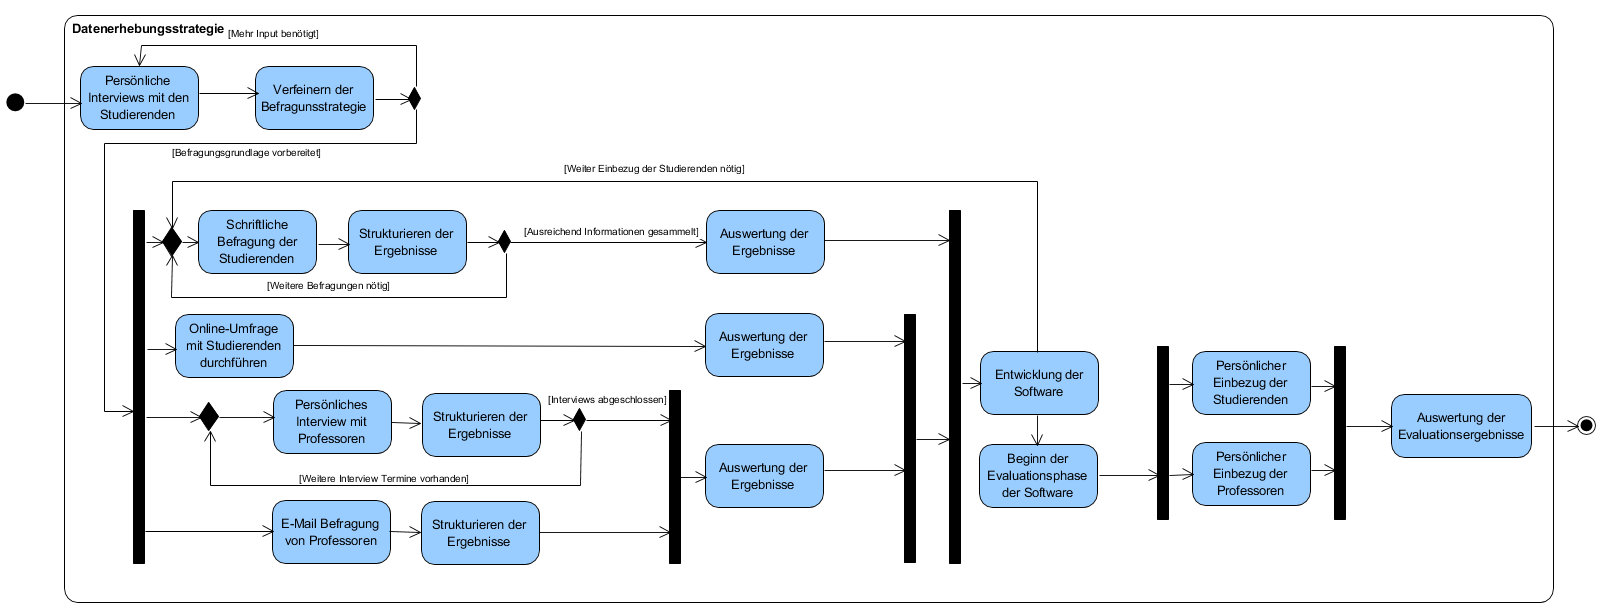
\includegraphics[scale=0.6, angle=90]{Bilder/Diagramme/AnalysestrategieDetails.png}
\end{center}

\newpage
\subsection{Transkripte der Interviews mit den Professoren}
\label{anhang:interviewProfessorenTranskripte}
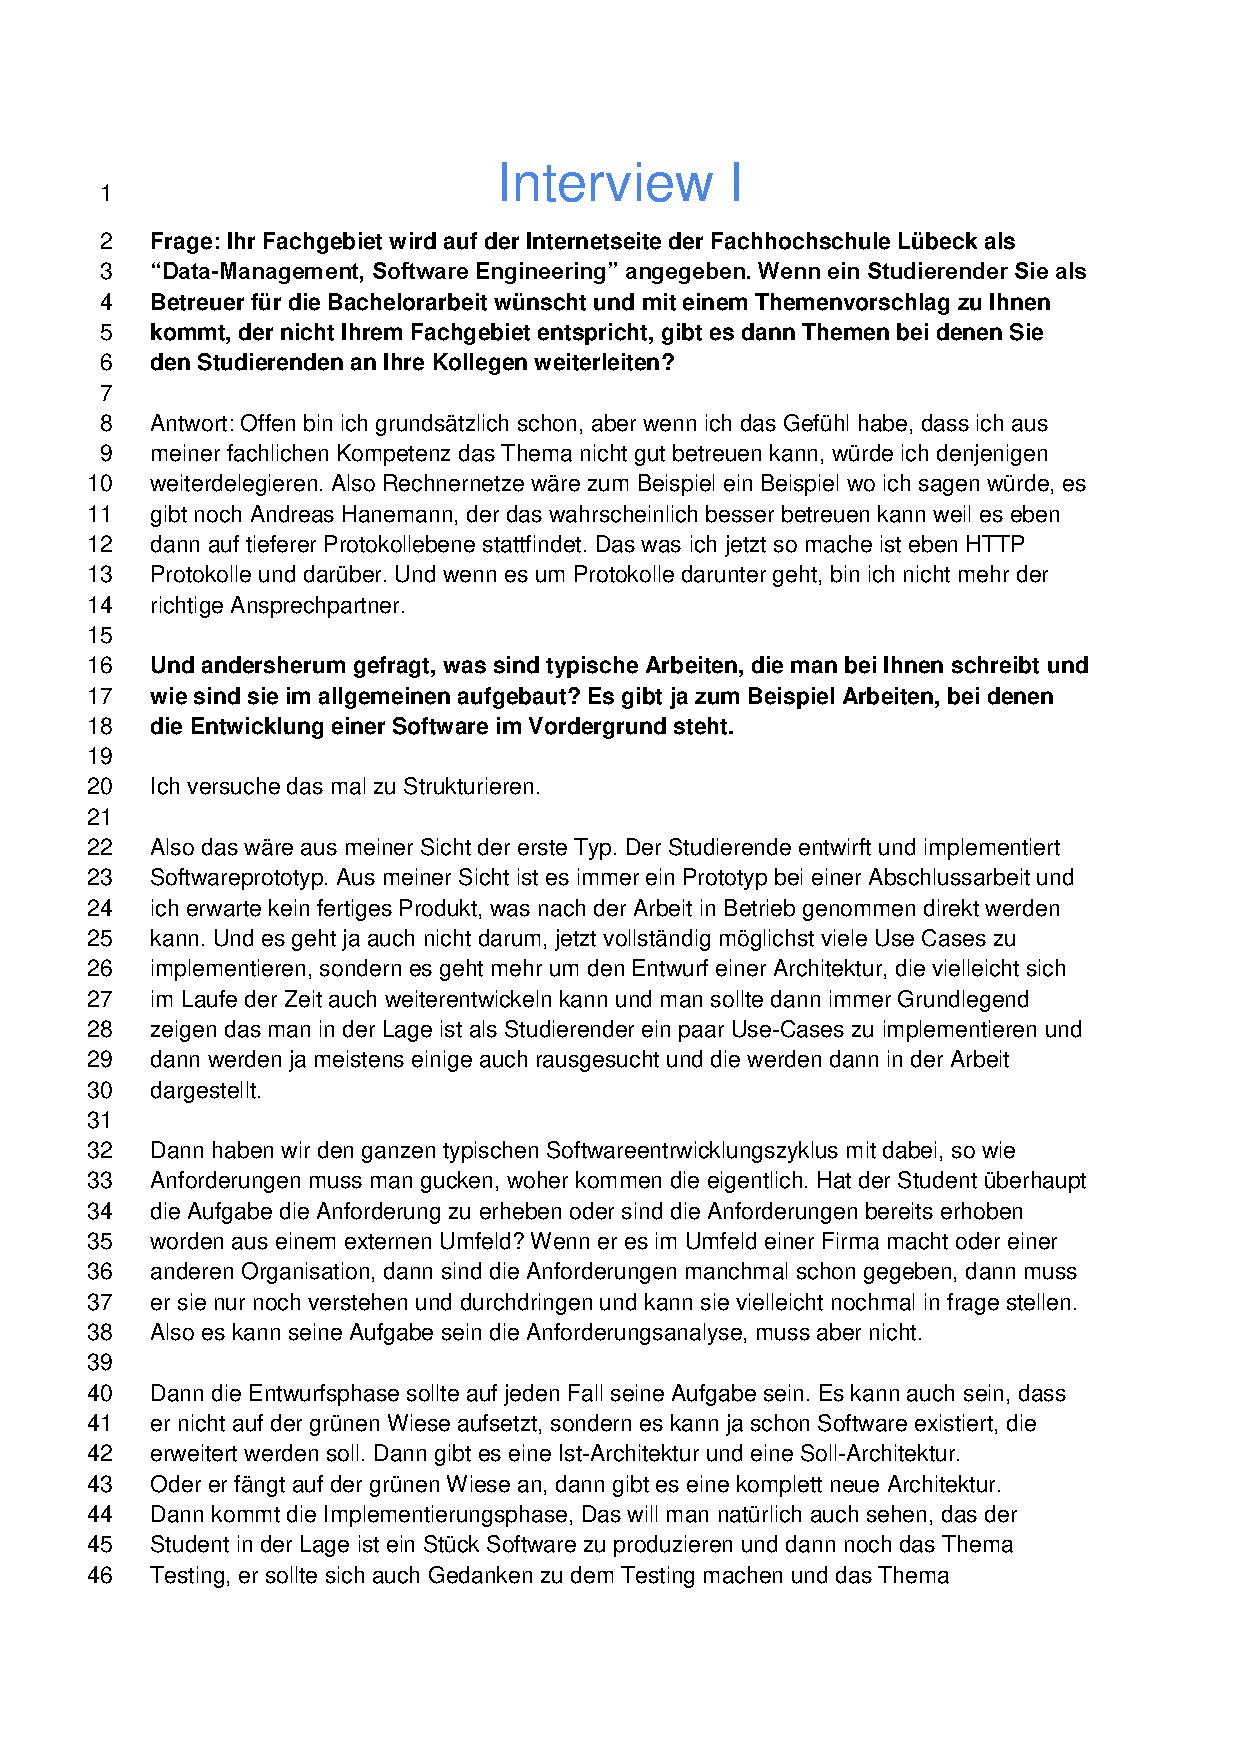
\includepdf[pages=-]{Anhang/Anforderungsanalyse/Professoren/Persoenliche_Interviews/Aufzeichnungen/Interview_I.pdf}

\includepdf[pages=-]{Anhang/Anforderungsanalyse/Professoren/Persoenliche_Interviews/Aufzeichnungen/Interview_II.pdf}
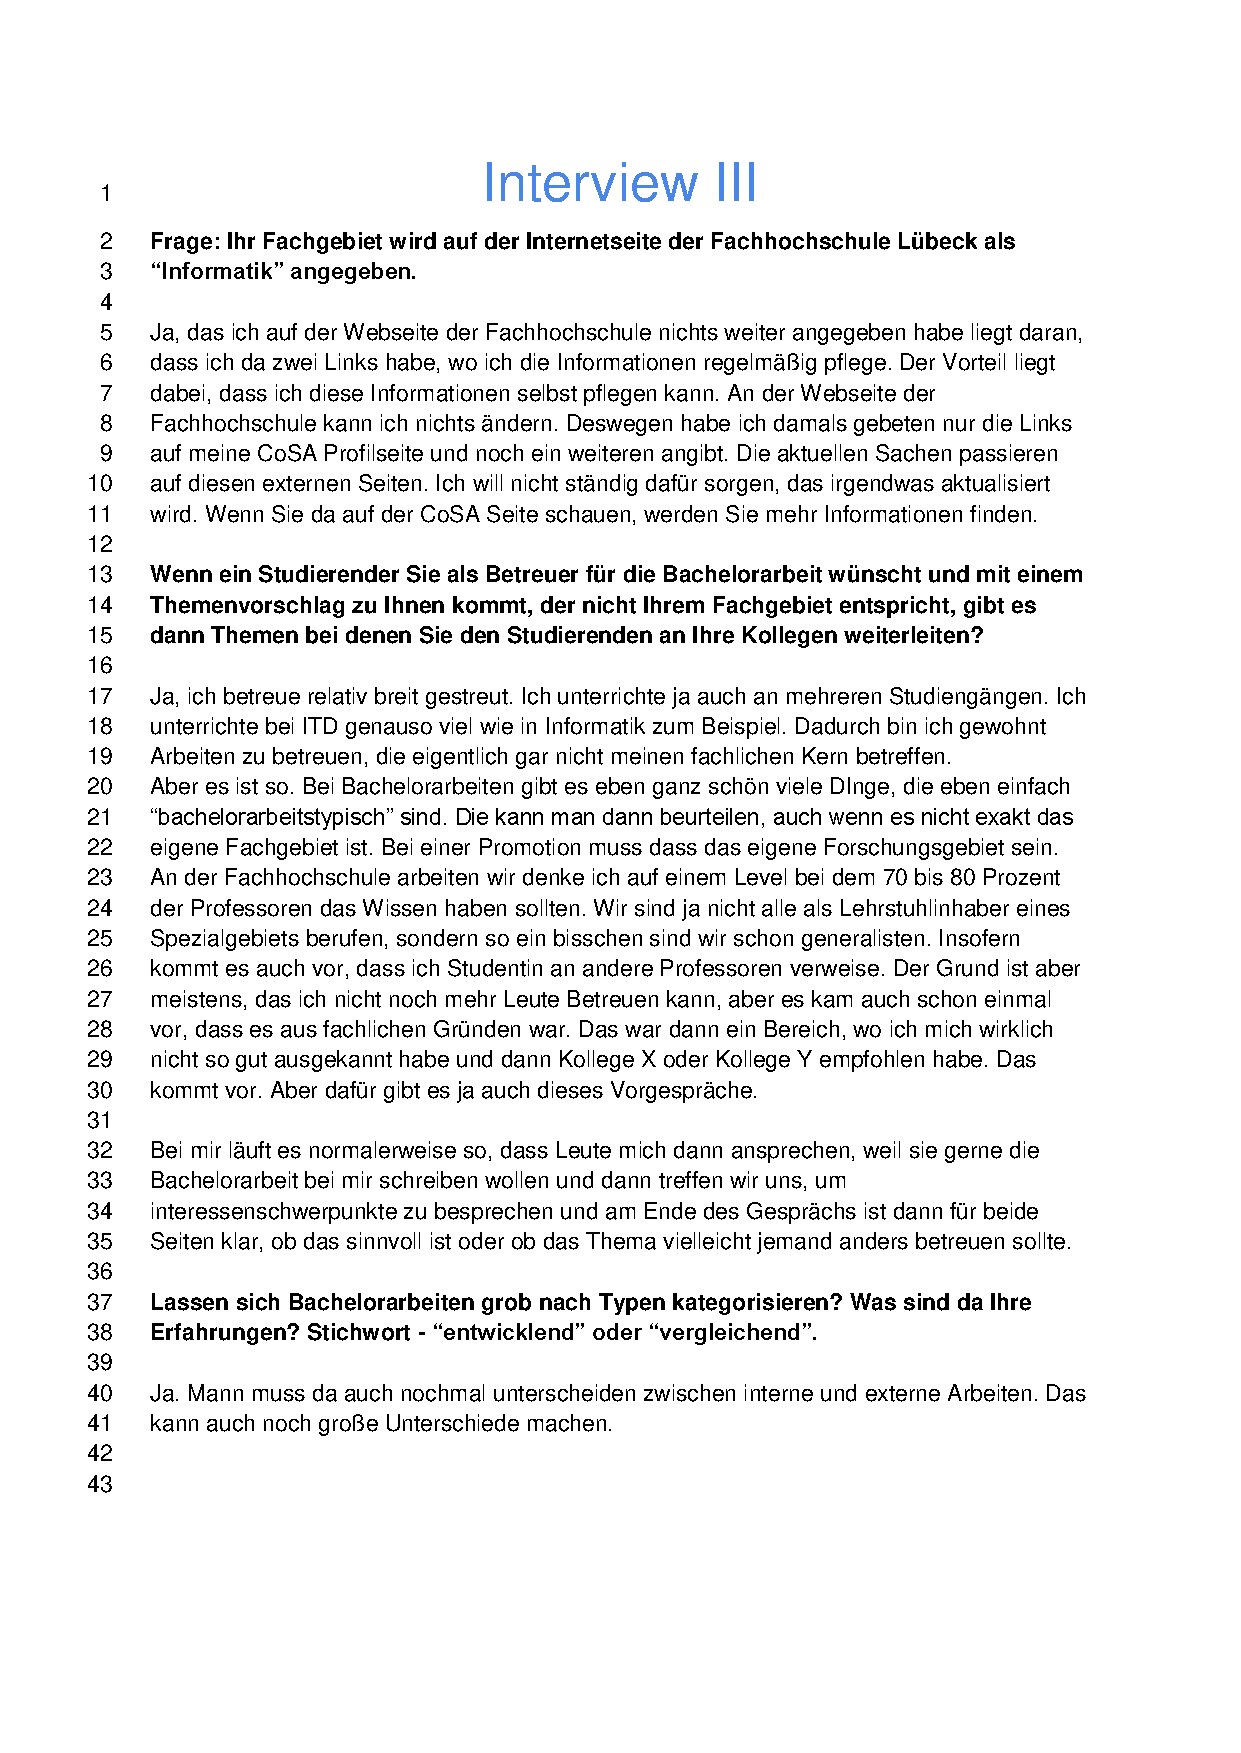
\includepdf[pages=-]{Anhang/Anforderungsanalyse/Professoren/Persoenliche_Interviews/Aufzeichnungen/Interview_III.pdf}
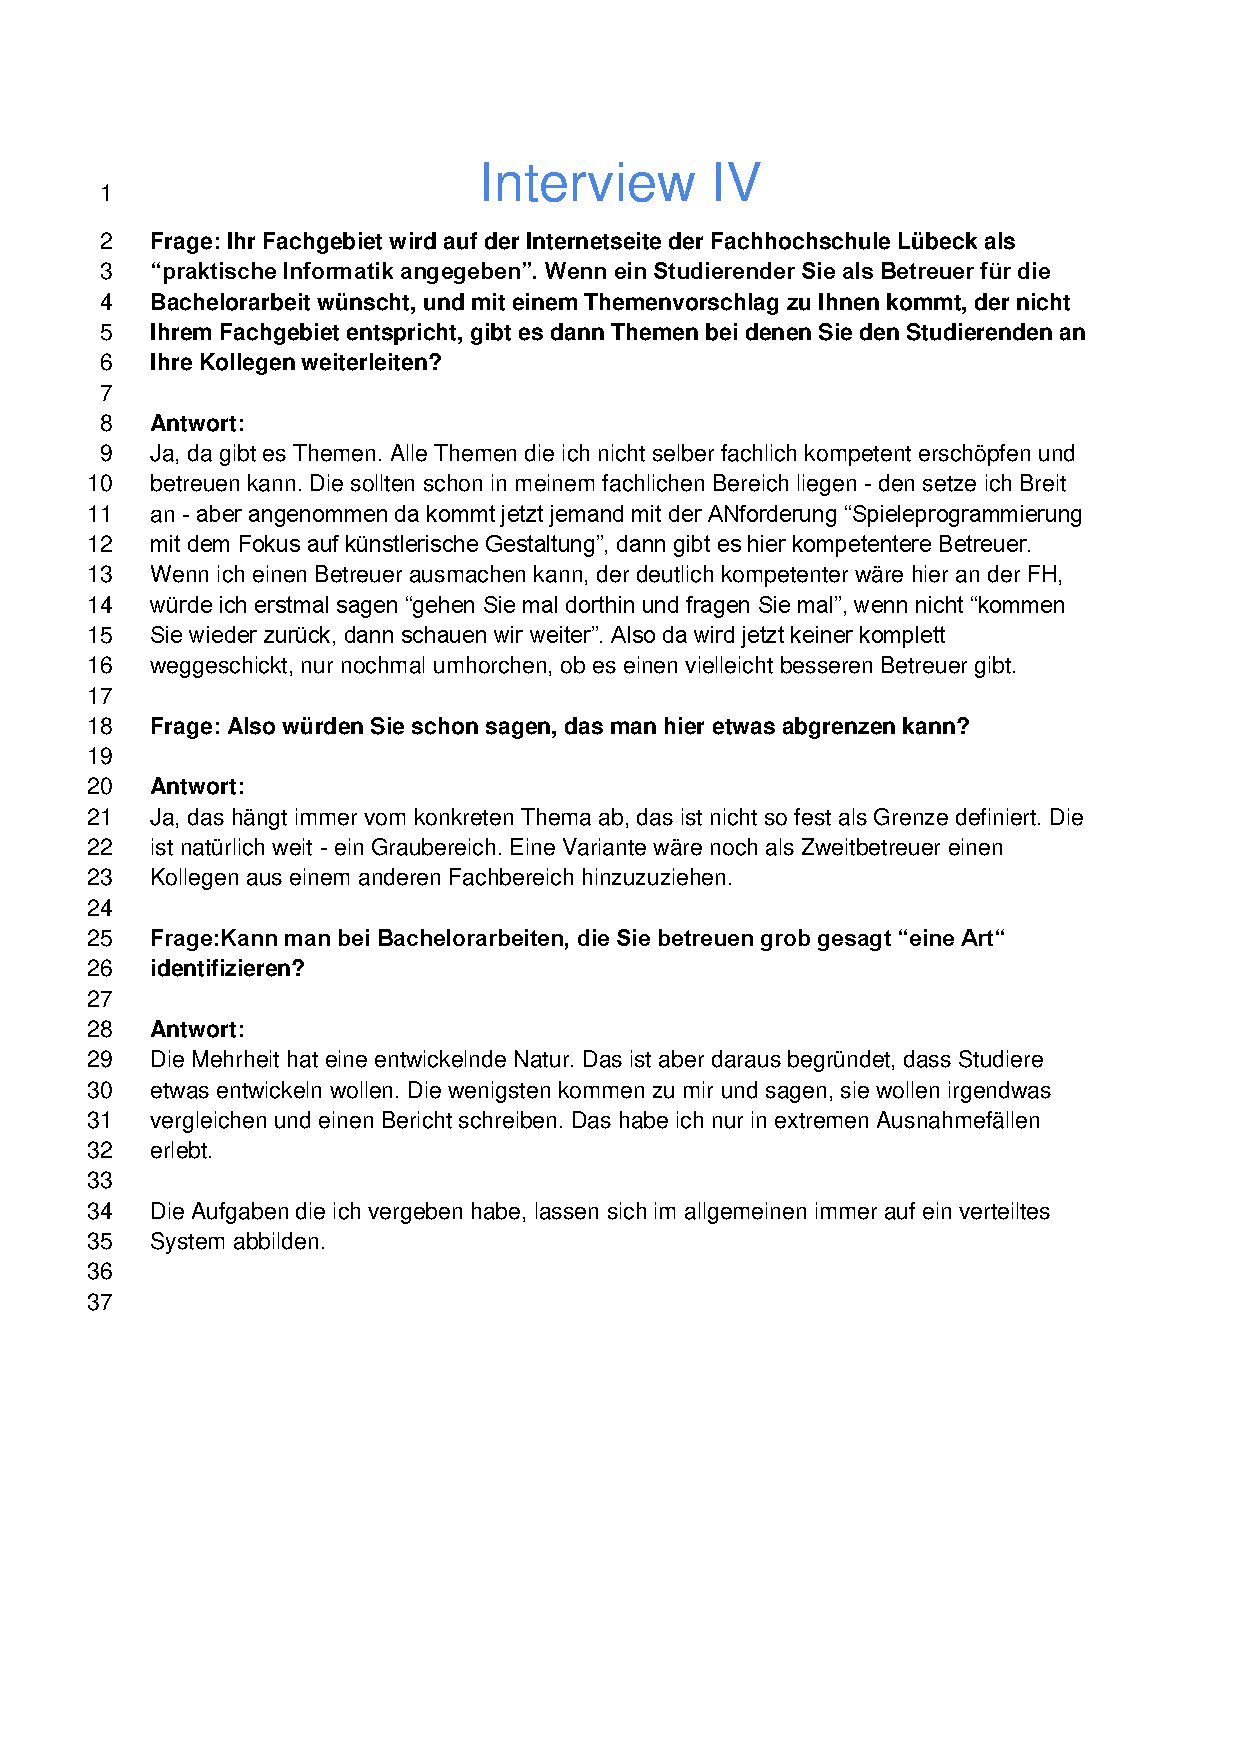
\includepdf[pages=-]{Anhang/Anforderungsanalyse/Professoren/Persoenliche_Interviews/Aufzeichnungen/Interview_IV.pdf}
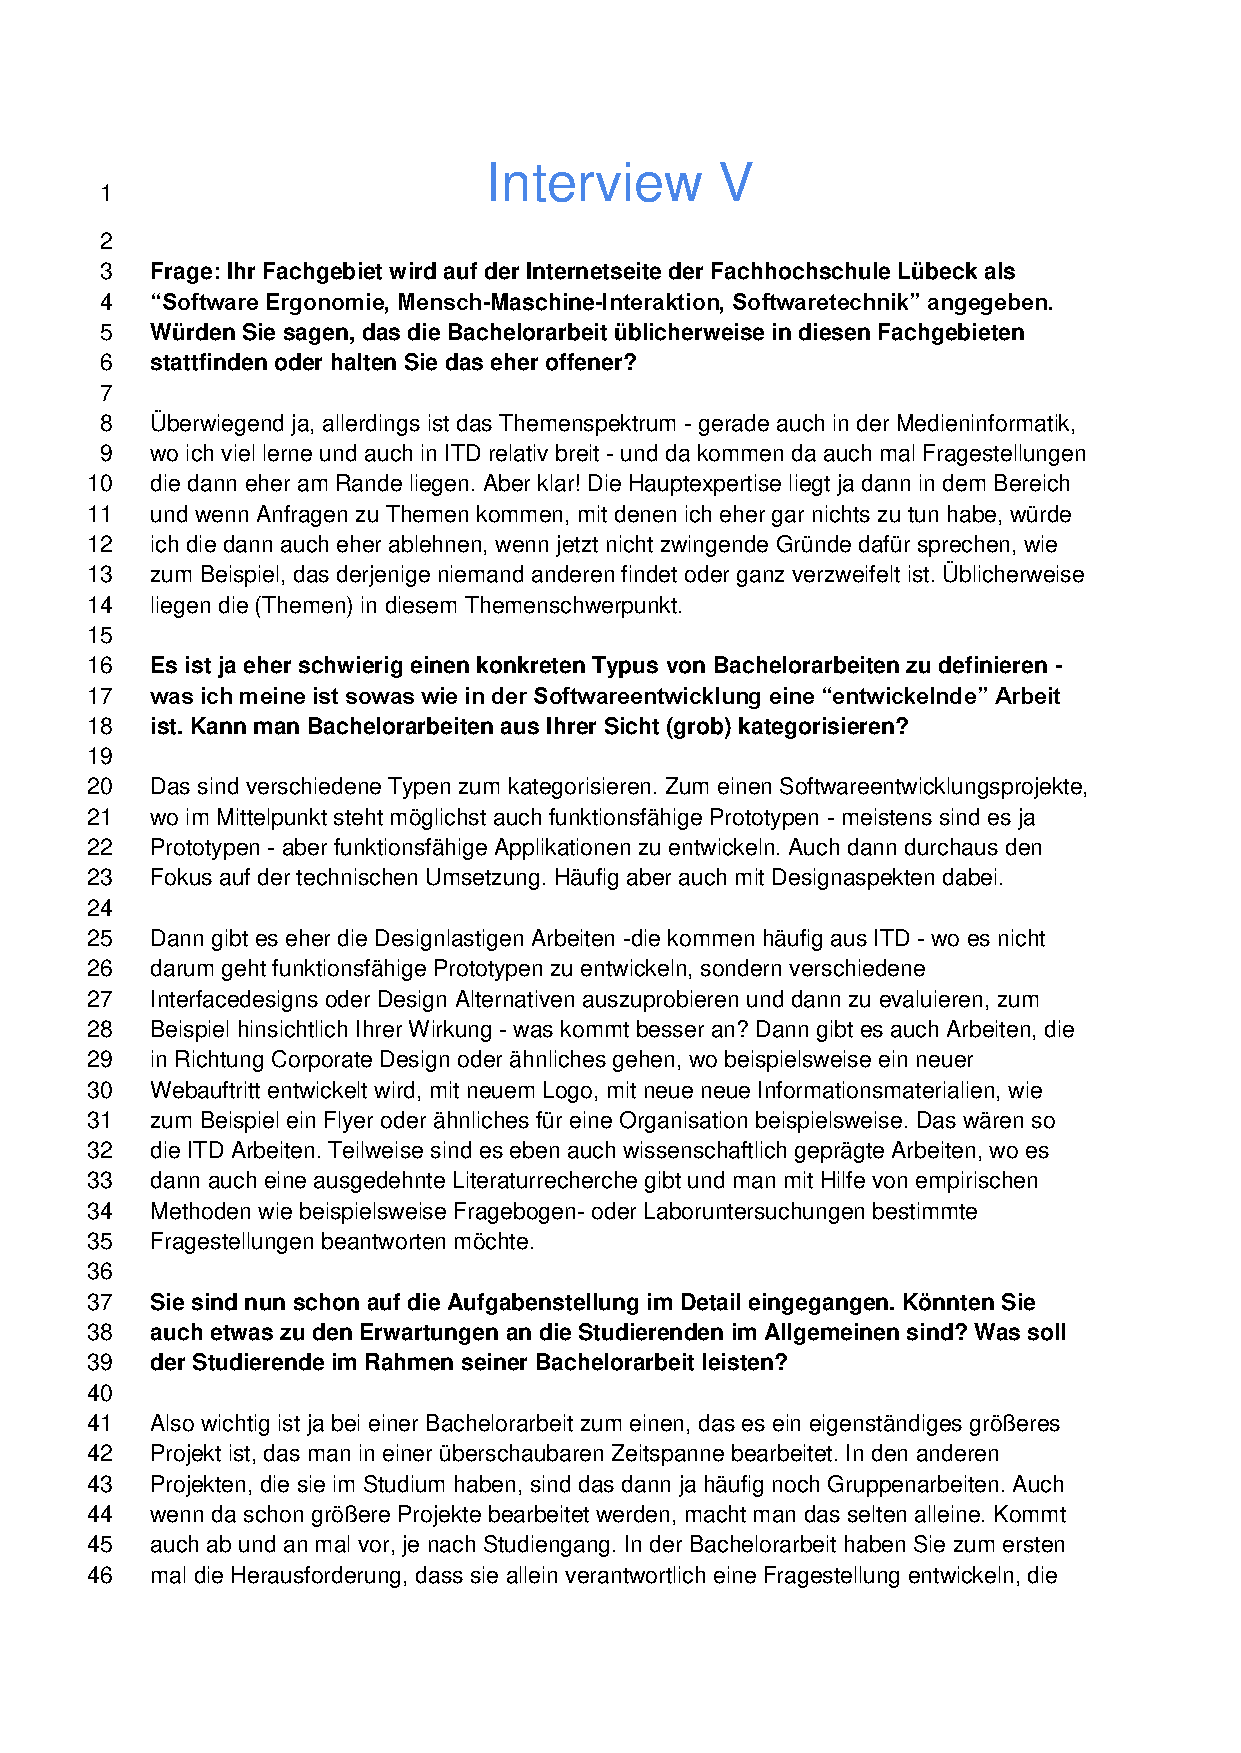
\includepdf[pages=-]{Anhang/Anforderungsanalyse/Professoren/Persoenliche_Interviews/Aufzeichnungen/Interview_V.pdf}

\newpage
\subsection{Auswertung der Ergebnisse der Interviews mit den Professoren}
\label{anhang:interviewProfessorenAuswertung}

\includepdf[pages=-]{Anhang/Anforderungsanalyse/Professoren/Persoenliche_Interviews/Auswertung/Interview_Auswertung_der_Professoren.pdf}

\newpage
\subsection{Zusammenfassung der schriftlichen Befragung der Studierenden}
\label{anhang:schriftlicheBefragungStudierendeZusammenfassung}
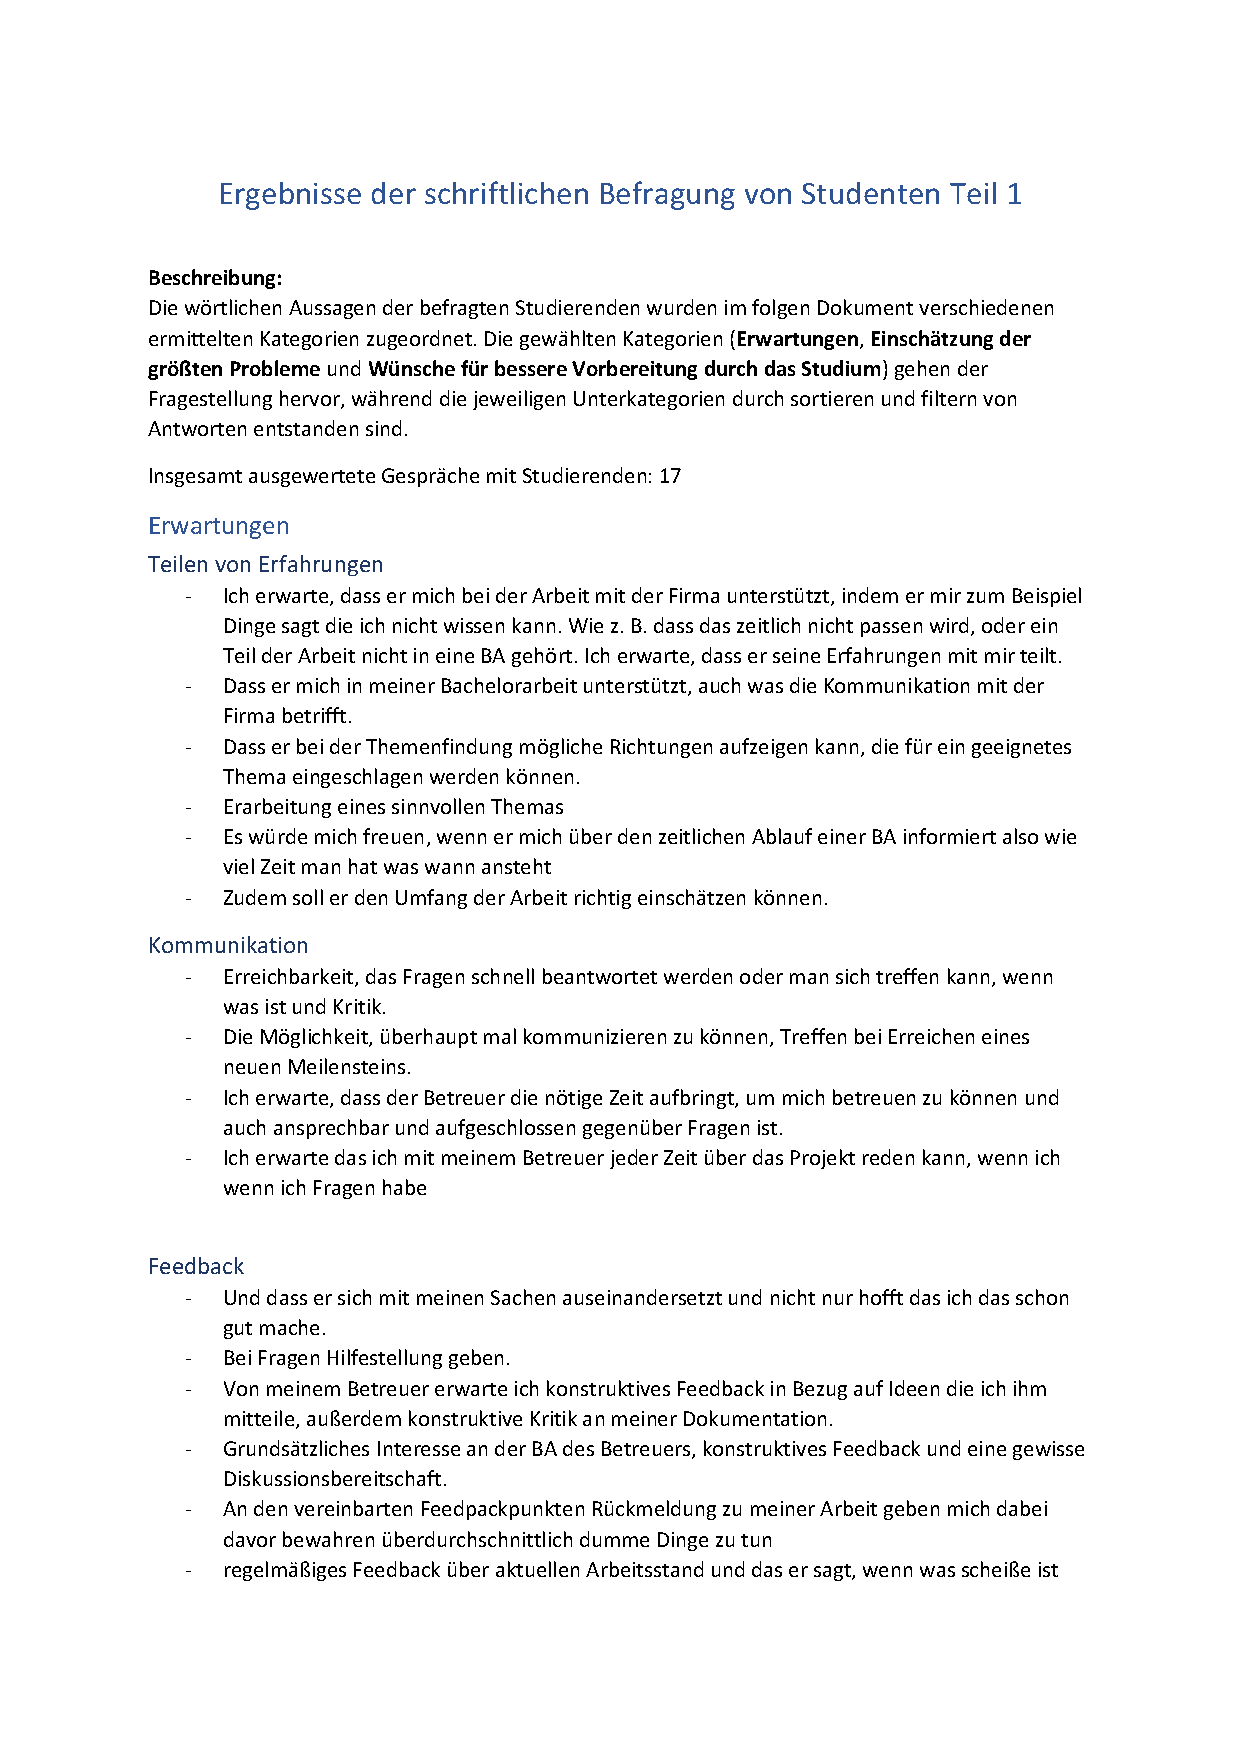
\includepdf[pages=-]{Anhang/Anforderungsanalyse/Studenten/Schriftliche_Befragung/Ergebnisse_der_Befragung.pdf}

\newpage
\subsection{Ergebnisse der Online-Umfrage für die Studierenden}
\label{anhang:onlineUmfrageStudierendeErgebnisse}
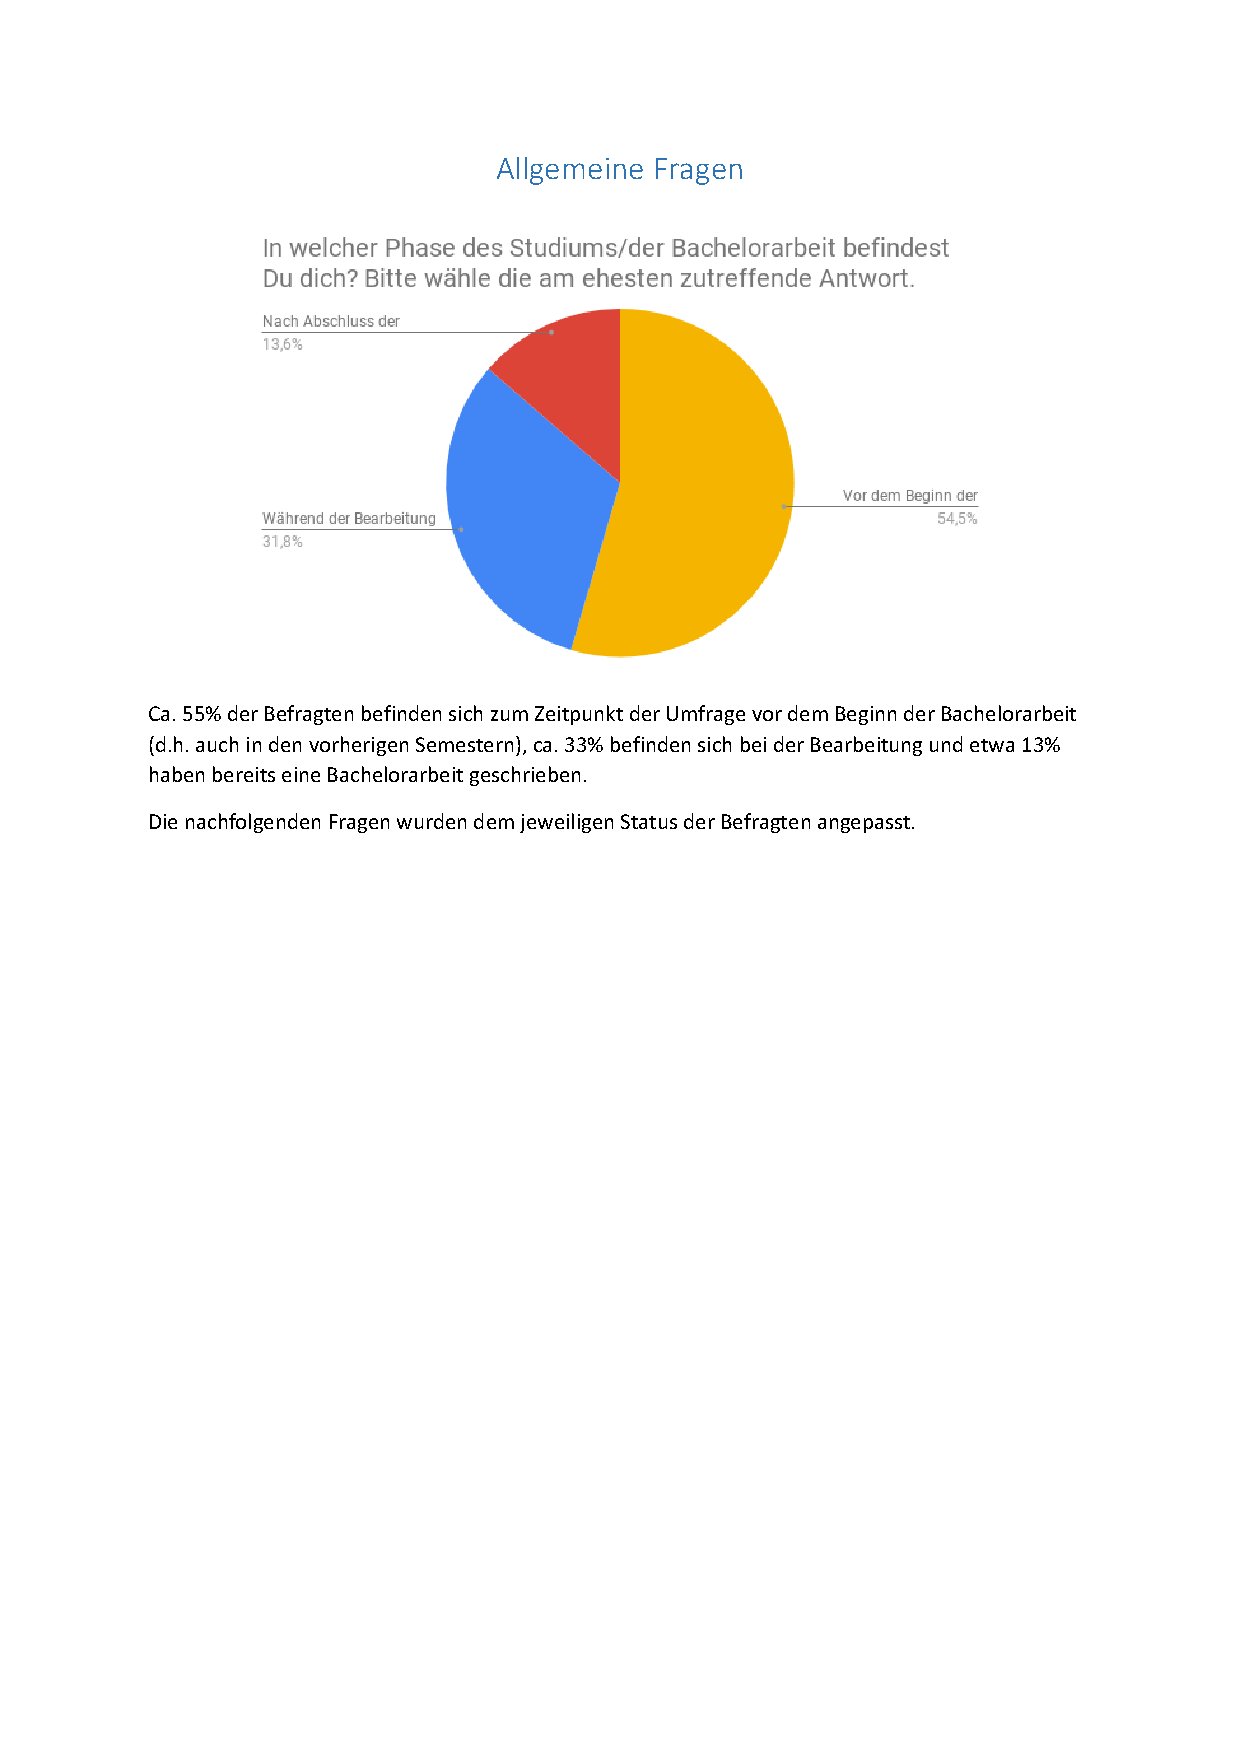
\includepdf[pages=-]{Anhang/Anforderungsanalyse/Studenten/Umfrage/Auswertung_Umfrage.pdf}

\end{document}
